% Template for SE Project software documentation
% (c) Farhad Mehta 2021

\documentclass[11pt, oneside, a4paper]{book}

% File containing the commands and definitions
% that are used throughout this project.

\usepackage[english]{babel}

% Set input encoding
\usepackage[utf8]{inputenc}

% For creating coloured text and backgrounds
\usepackage[table,xcdraw]{xcolor}

% For creating compact lists
\usepackage{paralist}

% To get the current date and time
\usepackage{datetime2}

% For including graphics
\usepackage{graphicx}

% For including captions
\usepackage{caption}

% For including .pdf files
\usepackage{pdfpages}

% For aligning Images (left, right center)
\usepackage[export]{adjustbox}

% For creating file-like structure
\usepackage{forest}

% Custom commands

\newcommand{\todo}[1]{TODO: {#1}}

% The following command indicates that its content consists of instructions
% Even if it does not do anything, it is still a good idea to keep instructions within the `instruction` tag to separate them from the rest of the text. One could then typeset them differently, or choose to remove them form the document by redefining the command definition 
\newcommand{\instructions}[1]{#1}

% Uncomment the following command to remove all instructions
% \newcommand{\instructions}[1]{}

% Uncomment the following to make instructions appear in coloured boxes
% Note: The changes within `\instruction` are not visible in latexdiff when they are typeset in this way
% \usepackage{tcolorbox}
% \newcommand{\instructions}[1]{
%     \begin{tcolorbox}[sharp corners, colback=green!30, colframe=green!80!blue, title=Instructions]
%         #1
%     \end{tcolorbox}
% }

% Uncomment the following to make instructions appear in colour.
% Note: The changes within `\instructions` are not visible in latexdiff when they are typeset in this way
% \newcommand{\instructions}[1]{ { \color{blue} #1 } }

% Get a git version description roughly using the idea in  
% https://blog.wxm.be/2013/08/20/automated-git-commit-number-in-latex.html
% Note that the file that is included needs to be generated before the document is built.
% Refer to the makefile for further details.
\IfFileExists{../gitDescription.tmp}
{\newcommand{\gitDescription}{\input{../gitDescription.tmp}}}
{\newcommand{\gitDescription}{Not available}}

% Note: Importing hyperref must be done towards the end since it
% redefines many macros
%
% Note:
%  The following packages must be imported *before* hyperref:
%  
%  The following packages must be imported *after* hyperref:
%    amsrefs, geometry
\usepackage{hyperref}

\usepackage{geometry}

% options for package geometry (influences writable area on page)
% \geometry{a4paper, top=2cm, bottom=2cm}

\usepackage{csquotes}
\usepackage[style=verbose-note]{biblatex}


\usepackage{subfig}

\usepackage{fancyvrb}

\usepackage{dirtree}


\hypersetup{
    pdfauthor={Farhad Mehta, Thomas Kälin},
    pdftitle={Template for SE Project software documentation},
    colorlinks=true,
    linkcolor=blue,
    filecolor=magenta,      
    urlcolor=cyan,
    pdftitle={Overleaf Example},
    pdfpagemode=FullScreen,
}

\addbibresource{./bibliography.bib}

\begin{document}
\pagestyle{empty}

\frontmatter

\begin{titlepage}

    \begin{center}

        \fbox{\Huge Bachelor Thesis}

        \vspace{1 cm}

        {\Large Project Documentation} \\

        \vspace{0.5cm}

        {\Huge Haskell Substitution Stepper}

        \vspace{0.5cm}

        Semester: Spring 2023

        \vspace{1 cm}

        
\includegraphics[scale=0.1]{resources/haskell-logo.png}

        \vspace{1 cm}

        Date: \DTMnow \\
        \vspace{1 cm}

        \begin{tabular}{rl}
            \textbf{Author:}    & Carlo Del Rossi \\
            \textbf{Project Advisor:} & Prof. Dr. Farhad D. Mehta \\
            \textbf{Co-Examiner:}     & Dr. Joachim Breitner
        \end{tabular}

        \vfill

        
\includegraphics[height=2cm]{resources/ost-logo.png}\\

        \vspace{1cm}
        School of Computer Science\\
        OST Eastern Switzerland University of Applied Sciences

    \end{center}

\end{titlepage}

\chapter*{Abstract}

With functional programming languages becoming more widespread and being taught at Universities,
many programmers will eventually get in contact with them.
Since functional programs can be very different from imperative ones,
especially due to the heavy reliance on recursion,
this could be very interesting for all the people that are not yet familiar with Haskell's concepts.

\ \\
While functional languages like Haskell have debuggers,
they are not as user-friendly and don't offer as much insight as debuggers for imperative languages.
The internal state of the program is usually not displayed very comprehensibly,
which leads to the not being very useful for learning processes.

\ \\
The goal of the Haskell Substitution Stepper is to provide the user with the capability to step through a Haskell program
and to be able to see what happens in the background when a function is executed.
This is supposed to solve the usability problems that the regular Haskell debugger has.

\ \\
For this, we came up with an application where the user can specify a function that he would like to step through
and the application would load this function and then use Haskell's rules to step through.
The user can see the whole internal state of the term that is being stepped through
and the highlighting of the changes makes it easy to see what happens in each step.
The user can choose between different modes of derivation and can control the flow of the derivation.
The addition of helpful commands also allows the user to skip certain parts of the derivation that might not be interesting to them.

\tableofcontents

\mainmatter

\part{Introduction}
\chapter{Management Summary}

\instructions{
    
    Das Management Summary (auch Lay Summary) richtet sich an ein breites Publikum und an das
    Management, welches in der Regel über keine Fachkenntnisse im bearbeiteten Thema verfügen. Das
    Management Summary soll kurz und verständlich beschreiben, worum es bei der Arbeit geht und welche
    Ergebnisse erzielt wurden. Die Sprache soll knapp, klar und stark untergliedert sein. Der Umfang beträgt in
    der Regel 2-3 (max. 5) Seiten. Bilder sind hier im Gegensatz zum Abstract erwünscht.
    Beispiel Gliederung für Management Summary:
}


\part{Analysis}
\chapter{Domain Analysis}

\section{Problem}

\section{Domain Specific Language}

\section{Domain Model}

\section{Domain Model Assumptions}

\chapter{Requirements}

\section{Functional Requirements}

The following table lists the identified functional requirements.
The MVP includes FR1, FR3, FR4, FR5, and FR6.

\begin{table}[h!]
    \makebox[\textwidth][c]{
        \begin{tabular}{ p{1.5cm} p{12.65cm}}
            \textbf{FR} & \textbf{Description} \\ \hline \\                                                                                                                                                                              
            \textbf{FR 1} & The user can specify functions that should not be stepped through and instead derived in a single step. \\
            \textbf{FR 2} & The user can control the derivation flow in such a way, that they can skip the derivation for certain redexes interactively. \\
            \textbf{FR 3} & The user can step through the reduction line by line. \\
            \textbf{FR 4} & The user can make the derivation run through to the end without requiring any interaction. \\
            \textbf{FR 5} & The tool supports a verbose variant, that indicates which function has been applied. \\
            \textbf{FR 6} & The user can import user-defined files and step through functions defined in these files. \\
        \end{tabular}
    }
    \label{tab:functionalRequirements}
\end{table}

\section {Non-Functional Requirements}

This section contains the NFRs, that are prioritized from 1 to 3, where 1 is the highest priority and 3 the lowest.

\begin{table}[h!]
    \makebox[\textwidth][c]{
        \begin{tabular}{ |p{1.3cm} |p{7cm} |p{7cm} |p{0.85cm}|}
            \hline
            \textbf{Nr.} & \textbf{Description} & \textbf{Measurement}  & \textbf{Prio} \\ \hline                                                                        
            NFR1         & The tool is usable for people with little experience in functional programming.  & The derivation of a user-defined function takes max. one import command and one step command. The function is defined in one file and depends only on other functions in the same file. &  1 \\ \hline
            NFR2         & The tool provides an open API or CLI, to open it up to additional UIs. & & 3 \\
            \hline
        \end{tabular}
    }
    \label{tab:NFRs}
\end{table}


\part{Design}
\chapter{Architecture}
This chapter highlights the architecture of the Substitution Stepper as well as the reasoning for some big decisions.

\section{Overview}
The Substitution Stepper consists of multiple logically grouped folders that each have a specific responsibility.
The most important folders/modules are shown in Figure \ref*{fig:architecture},
though not all of them are shown in full detail as that would clutter up the diagram too much and would not provide a lot of value.

\begin{figure}[ht!]
    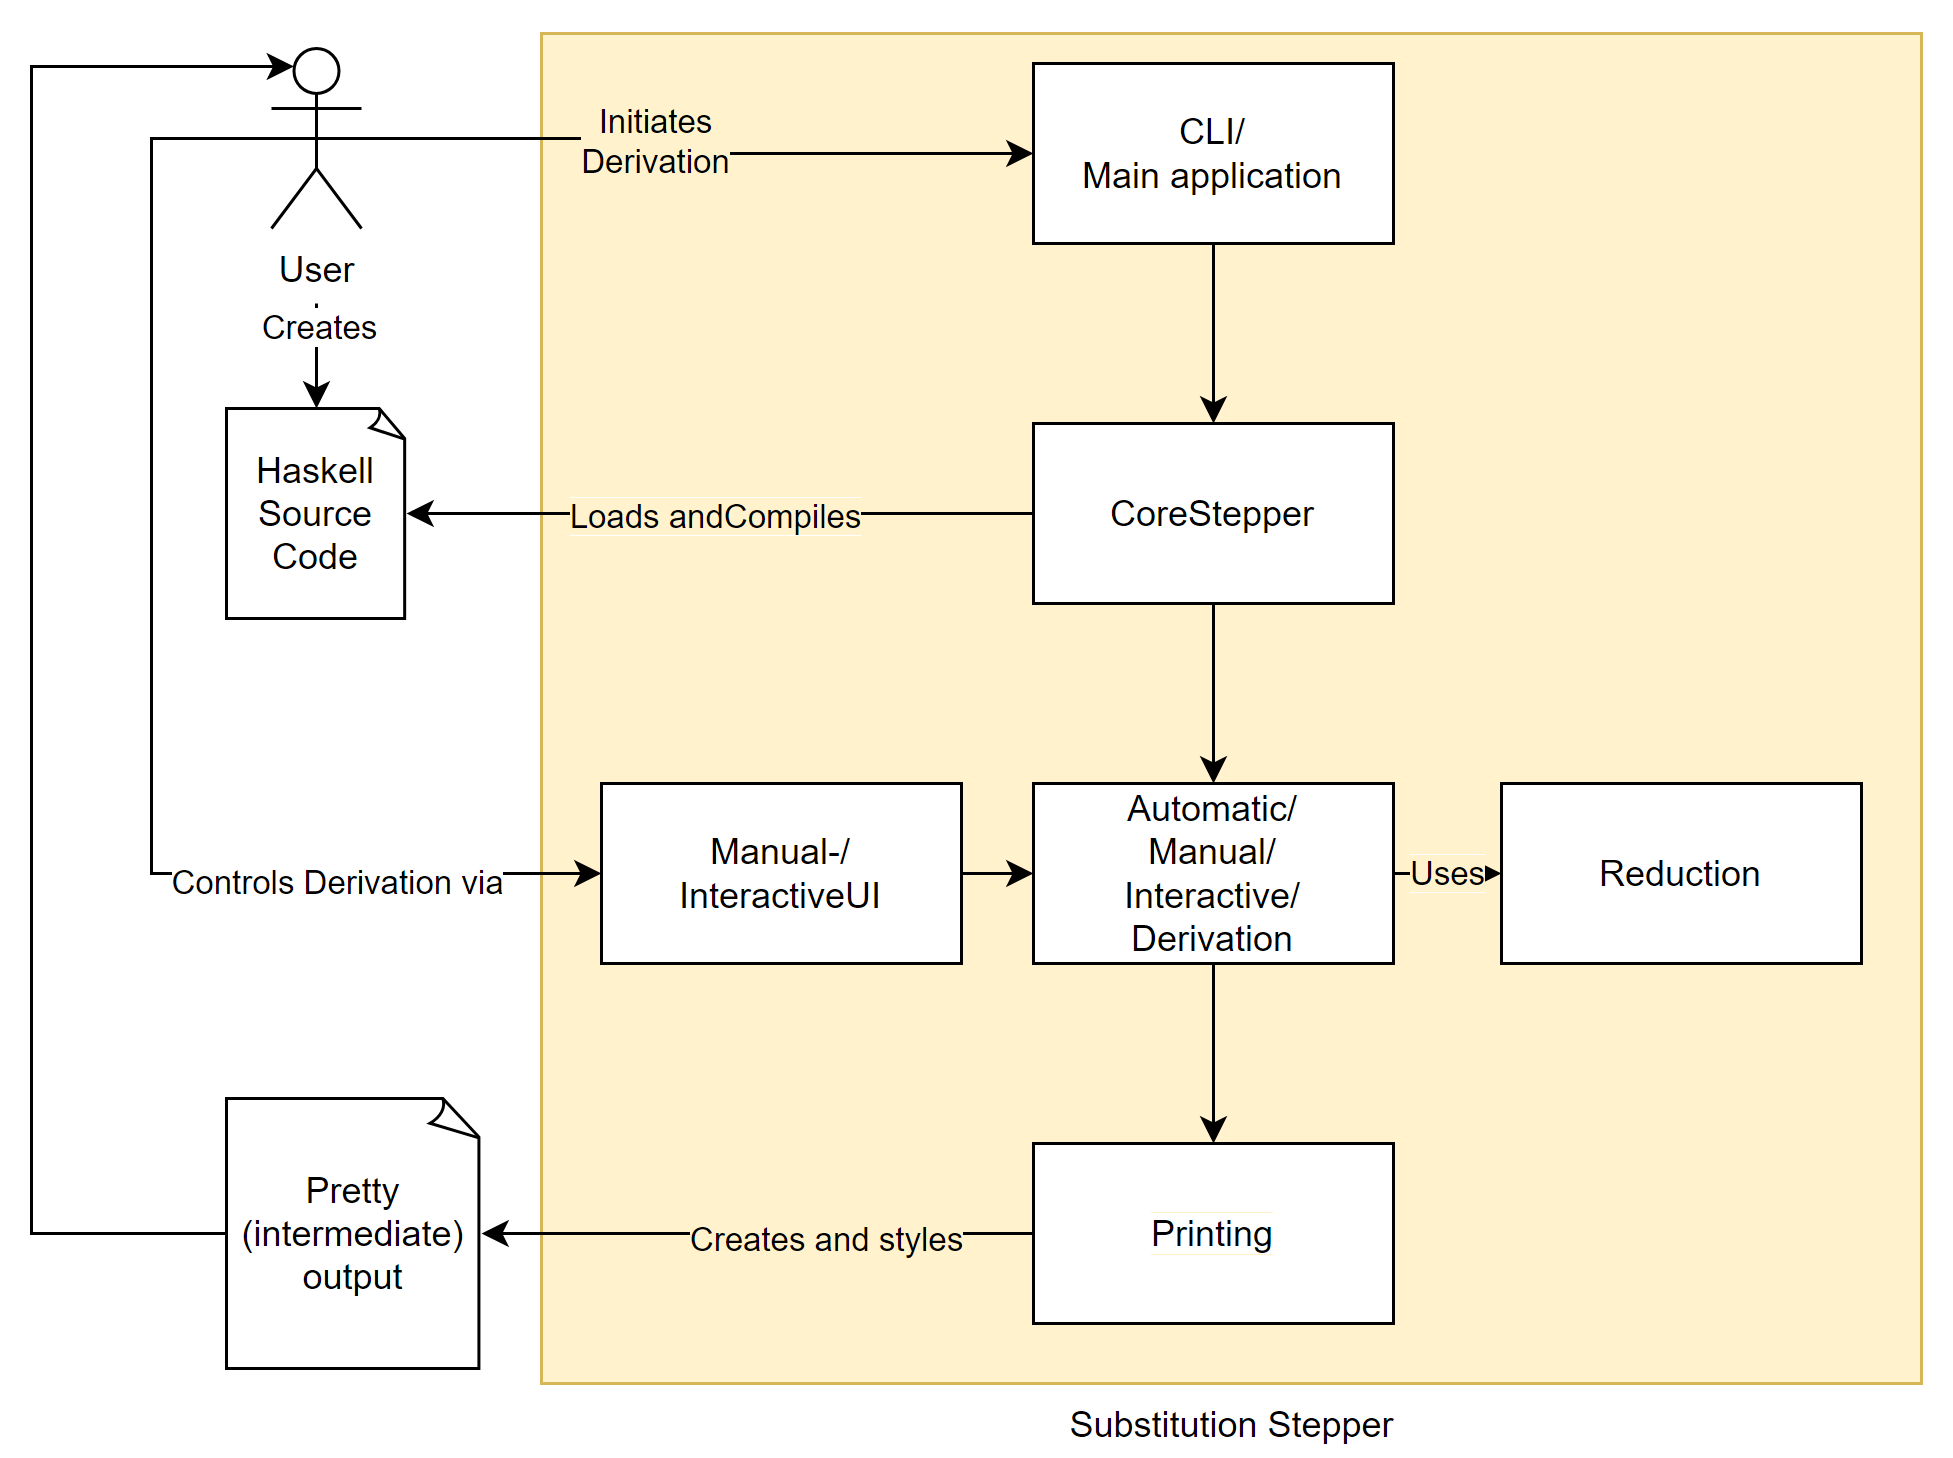
\includegraphics[width=1\textwidth]{resources/Architecture.PNG}
    \caption{Architecture of the Substitution Stepper}
    \label{fig:architecture}
\end{figure}

\subsection{Main application}
The main application is responsible for initiating the derivation.
The module AppConfig is used by the main application to extract the relevant arguments from the command line,
based on which the derivation is initiated.
The AppConfig module is also responsible for adding default values for arguments that were not passed to the application.

\subsection{CoreStepper}
The CoreStepper module, which was developed outside of the scope of this thesis,
takes Haskell source code and compiles it to GHC Core code.
All bindings from the stepped module are collected and returned.
The binding for the stepped function is fetched as well and passed to the Derivation module via the main application.

\subsection{Derivation}
The module \texttt{Derivation.DerivationUtils} is used by the main application to prepare the GHC Core code for stepping.
The function \texttt{instantiateDerivation} is used to create all the delta reduction rules and to get the term that will be derived.
With this done, the respective derivation mode can be initialized.
Based on which derivation mode is desired by the user,
the control flow is passed on to the \texttt{Derivation.Automatic}, \texttt{Derivation.Manual} or \texttt{Derivation.Interactive} module.
The stepping functionality,
defined in the \texttt{Derivation.Stepper} module,
relies on the contents of the \texttt{Derivation.Reduction} folder to execute the steps.
If the derivation is executed in manual or interactive mode,
the \texttt{UI.ManualUI} or \texttt{UI.InteractiveUI} module is used for the interaction with the user.

\subsection{Printing}
The modules contained in the \texttt{Printing} folder are used to display the GHC Core code to the user in a prettier and more Haskell-like way.

\section{Architectural Decisions}

\subsection{Derivation Logic}
For the derivation logic,
I have decided to go for a self-written set of derivation rules over the derivation logic that was provided by the \texttt{CoreStepper} module.
This gives me more control over the rules I want to feature,
and makes it easier for me to add functionality that is missing in the \texttt{CoreStepper} module like classes and instance functions.
However, it comes at the cost of having to put in more time to get a working set of derivation rules.
Since I value the flexibility that my self-written implementation gives me,
I chose the former option.

\subsection{Application Type}
For the application type,
I have decided to go for a command-line application over a GUI application like for example a VSCode extension.
The advantage of a command-line application is that it is simpler to implement
since there is no need to familiarize myself with the details of how to create a VSCode extension or similar.
On the other hand,
it takes more effort to make the interaction with the command line intuitive
and it takes some thought about how to best display the information so that the user understands what is going on.
Since I value the time-saving aspect of the first option,
especially because this Thesis is done as individual work,
I decided to go for a command-line application.

\subsection{Sharing}
Haskell's lazy evaluation makes use of sharing,
so the same expression doesn't have to be reduced multiple times despite using the leftmost outermost strategy.
For the Substitution Stepper, however,
I have decided to ignore this feature.
This removes the need for a heap containing all the evaluated expressions.
Since no heap is needed it is also easier to display the stepped terms and probably also less confusing for people who are new to Haskell.
Of course, this has the drawback of not being entirely accurate to the derivation strategy used by Haskell.
Despite the slight inaccuracy I went for the option without sharing,
as I value the simplicity of an approach without sharing more than the accuracy
and I think that it has more didactic value for Haskell newbies.

\chapter{UI Design}

This chapter contains the initial sketches for the design of the derivation UI with a CLI tool.

The derivation uses the following function definitions:

\begin{verbatim}
    data Nat = S Nat | Z

    double :: Nat -> Nat
    double Z = Z
    double (S n) = S (S (double n))

    (+) :: Nat -> Nat -> Nat
    Z + n = n
    (S m) + n = m + (S n)

    fib :: Nat -> Nat
    fib Z = S Z
    fib (S Z) = S Z
    fib (S (S n)) = fib (S n) + fib n
\end{verbatim}

\section{Base Variant}

The base variant of the tool automatically steps through the derivation without user interaction.

\begin{verbatim}
 > step double (S (S Z))

        S (S (double (S Z)))

        S (S (S (S (double Z))))

        S (S (S (S (Z))))
\end{verbatim}

\section{Verbose Variant}

The verbose variant is similar to the base variant.
The difference is that the verbose variant includes information about which function was applied during the step.
The previous derivation looks like the following in verbose mode:

\begin{verbatim}
> step -v double (S (S Z))
        = { applying double }
          S (S (double (S Z)))
        = { applying double }
          S (S (S (S (double Z))))
        = { applying double }
          S (S (S (S (Z))))
\end{verbatim}

\section{Hiding Variant}

The hiding variant allows the user to define functions, that should be derived in one step, thus hiding the details of the derivation.
The hiding variant can be used in combination with either the verbose or base variant.
An example of this can be seen in the following derivation (regular on the left side and hiding on the right side):

\begin{verbatim}
> step -v fib (S (S (S Z)))         | > step -v -s (+) fib (S (S (S Z)))
    ={ applying fib }               |     ={ applying fib }
      fib (S (S Z)) + fib (S Z)     |       fib (S (S Z)) + fib (S Z)
    ={ applying fib }               |     ={ applying fib }
      fib (S Z) + fib Z + fib (S Z) |       fib (S Z) + fib Z + fib (S Z)
    ={ applying fib }               |     ={ applying fib } 
      S Z + fib Z + fib (S Z)       |       S Z + fib Z + fib (S Z)
    ={ applying fib }               |     ={ applying fib }
      S Z + S Z + fib (S Z)         |       S Z + S Z + fib (S Z)
    ={ applying (+) }               |     ={ skipping (+) }
      Z + S (S Z) + fib (S Z)       |       
    ={ applying (+) }               |
      S (S Z) + fib (S Z)           |       S (S Z) + fib (S Z)
    ={ applying fib }               |     ={ applying fib }
      S (S Z) + S Z                 |       S (S Z) + S Z
    ={ applying (+) }               |     ={ skipping (+) }
      S Z + S (S Z)                 |
    ={ applying (+) }               |
      Z + S (S (S Z))               |
    ={ applying (+) }               |
      S (S (S Z))                   |       S (S (S Z))
\end{verbatim}

As can be seen in the above derivation, the right side saves 3 trivial applications of (+).
This can help to make the derivation shorter and hide trivial or uninteresting derivations.

\section{Manual Variant}

The manual variant is similar to the previous variants.
The output can be the same as any of the previous variants, the difference here is that the user can step through the derivation manually.
So after entering the step command, the first line of the derivation is displayed.
The user can then advance the derivation with the enter key or other commands step by step.
With this variant, the user can skip parts of the derivation interactively and slowly step through.

In a second step, if possible, the redexes should be highlighted, allowing the user to skip certain redexes and go straight to the interesting derivations.
In this example, the redexes are underlined with the tilde symbol and assigned numbers, which can be used in commands like goto, which skips all derivation steps until the specified redex is reached.

\begin{verbatim}
> step -m -v fib (S (S (S Z)))
          fib (S (S (S Z)))
> enter
        ={ applying fib }
          fib (S (S Z)) + fib (S Z)
          ~~~~~~1~~~~~~   ~~~~2~~~~ -- Multiple redexes are marked
> goto 2                            -- Skip redex 1 and go directly to 2
        ={ goto 2 }
          S (S Z) + fib (S Z)
> enter
        ={ applying fib }
          S (S Z) + S Z
> enter
        ={ applying (+) }
          S Z + S (S Z)
> enter
        ={ applying (+) }
          Z + S (S (S Z))
> enter
        ={ applying (+) }
          S (S (S Z))
          
\end{verbatim}

Interactive commands could include commands like the following:
\begin{itemize}
    \item enter: advance one line
    \item goto x: skip ahead to redex x
    \item step x: advance x lines
    \item q/quit: cancel stepping/exit the stepper
    \item continue: continue the stepping until the end is reached
\end{itemize}

\part{Implementation}
\chapter{Quality Measures}

This chapter describes the various quality measures that were put in place to make sure that the code is as clean as possible and working as expected.

\section{Coding Guidelines}

\begin{itemize}
    \item General
    \begin{itemize}
        \item Code needs to be committed frequently with descriptive commit messages.
        \item Side effects should be avoided whenever possible.
        \item Comments may only be used if they are helpful.
        \item Global variables should be avoided if possible.
        \item Exceptions are preferred over error codes.
        \item Nesting should not be deeper than 2 levels.
        \item No duplicate code. (DRY)
        \item Functions should be kept short (less than 11 lines).
        \item Create feature branches, before every merge, tests must be run.
    \end{itemize}
    \item Formatting
    \begin{itemize}
        \item Line length should not exceed 120 characters.
        \item Style guide: ESLint + AirBnB
        \item Code must be auto-formatted before being committed.
        \item Code must pass all tests before being committed.
    \end{itemize}
    \item Naming
    \begin{itemize}
        \item Function names should be verbs.
        \item Class names should be nouns.
        \item Longer, more descriptive names are preferred over short ones.
        \item No abbreviations in names.
        \item No 1-character names.
    \end{itemize}
\end{itemize}

\section{Test Concept}

\section{Workflow}

Pipelines?


\part{Discussion}
\chapter{Results}

This chapter describes the achieved and not achieved goals, 
which are closely related to the FR and NFRs.

\instructions{
    Ergebnisse der Arbeit: Was wurde erreicht, was wurde nicht erreicht? Stellen Sie einen konkreten Bezug zu
    den Anforderungen (FA, NFA) her und verknüpfen Sie diese mit Ihren Ergebnissen. Bleiben Sie objektiv und
    nehmen Sie (noch) keine Wertung Ihrer Arbeit vor (siehe "Schlussfolgerungen").
    Ergebnisse der Arbeit: Was wurde erreicht, was wurde nicht erreicht? Stellen Sie einen konkreten Bezug zu
    den Anforderungen (FA, NFA) her und verknüpfen Sie diese mit Ihren Ergebnissen. Bleiben Sie objektiv und
    nehmen Sie (noch) keine Wertung Ihrer Arbeit vor (siehe "Schlussfolgerungen").
}

\section{Functional Requirements}

\section{Non-Functional Requirements}

\section{Screenshots}

\chapter{Conclusion \& Next Steps}

\instructions{
    Ergebnisdiskussion: In der Schlussfolgerung werden die Ergebnisse reflektiert und von Ihnen bewertet.
    Somit wird die Zielerreichung gemessen (Abgleich mit "Aufgabenstellung" und "Ziel der Arbeit") und ein
    Vergleich mit anderen/vorherigen Lösungen hergestellt. Die Schlussfolgerungen bilden einen wichtigen
    Abschnitt eines Berichts und sollen daher sorgfältig ausgearbeitet sein.

    Zudem erfolgt ein Ausblick auf mögliche Weiterentwicklungen, allfällige Verbesserungen oder neue
    Fragenstellungen, die sich aus Ihrer Arbeit ergeben.
    Fragen, die Sie sich selbst stellen können:
    \begin{itemize}
        \item Was wurde (Neues) erreicht?
        \item Was wurde nicht oder noch nicht genügend gut erreicht?
        \item  Was bleibt noch zu tun?
        \item  Welche neuen Fragestellungen ergeben sich aus Ihrer Arbeit?
    \end{itemize}
}

\section{Functional Requirements}

\subsection{Non-Functional Requirements}

\section{Reflection}

\section{Next Steps}


\part{References}
\listoffigures
\printbibliography[title=References]

\part{Appendix}
The following list is a brief overview of the Project Management.

\begin{itemize}
    \item \textbf{Project Planning Method: } Kanban
    \item \textbf{Long Term Plan: } see section Project Plan.
    \item \textbf{Short Term Plan: } available in \href{https://substep.atlassian.net/jira/software/projects/UI/boards/1/backlog}{Jira}
    \item \textbf{Risks: }
    \item \textbf{Time tracking: } available in \href{https://substep.atlassian.net/jira/software/projects/UI/boards/1/backlog}{Jira}.
\end{itemize}

\chapter{Project Plan \& Project Phase Description}

\section{Long-term Plan}

The long-term plan can be seen in Figure \ref*{fig:longTermPlan}.

\begin{figure}[!ht]
    \centering
    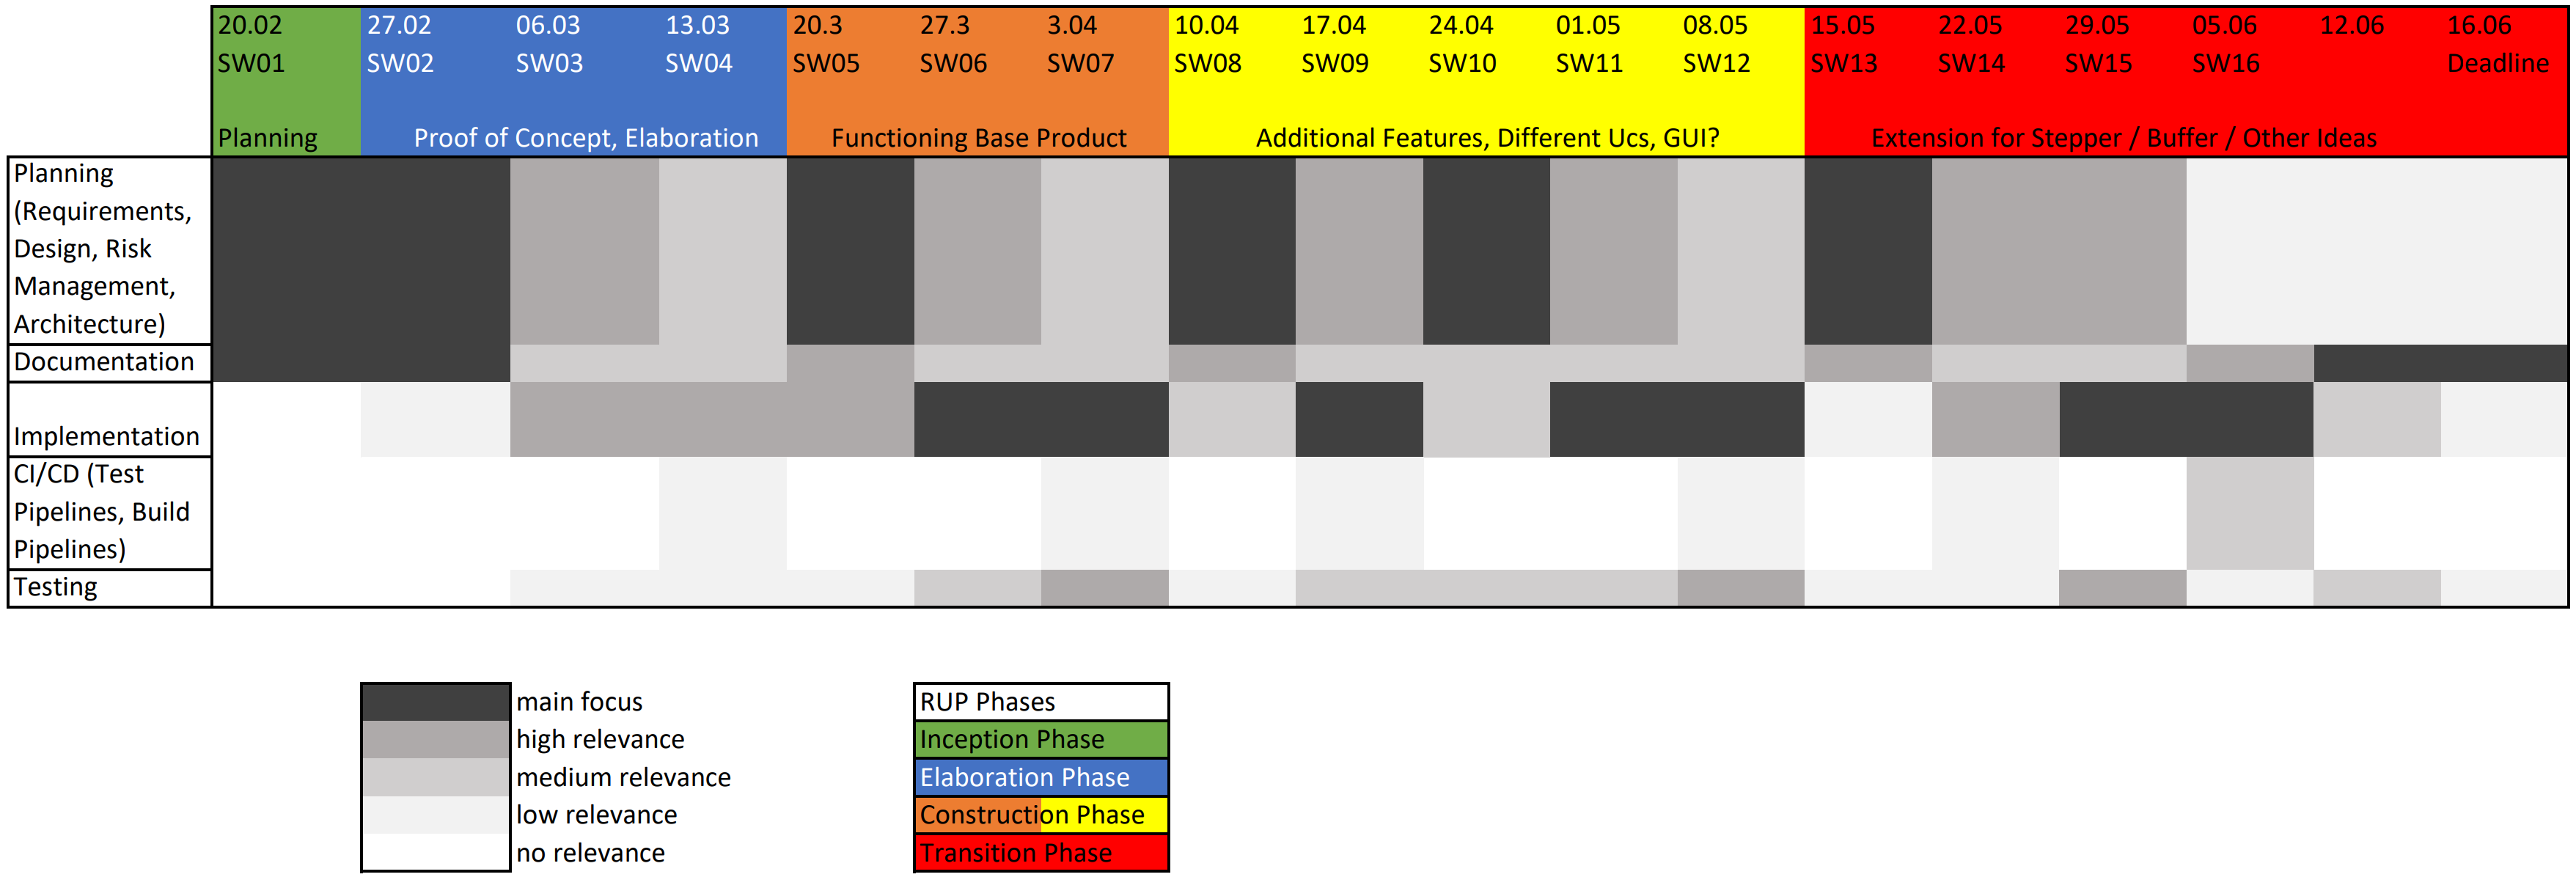
\includegraphics[width=0.96\textheight,angle=270]{resources/LongTermPlan.PNG}
    \caption{Long-Term Project Plan}
    \label{fig:longTermPlan}
\end{figure}

\clearpage
\section{Risk Management}

\subsection{Risks}

\begin{table}[!ht]
    \makebox[\textwidth][c]{
        \begin{tabular}{ p{2cm} p{8.15cm} p{2cm} p{2cm}}
            \textbf{Risk Nr.} & \textbf{Description} & \textbf{Probability} & \textbf{Severity} \\ \hline \\                                                                                                                                                                           
            \textbf{R1} & Unfamiliar Technology (f.ex. Haskell Core) & 2 & 3 \\
            \textbf{R2} & Sickness & 1 & 2 \\
            \textbf{R3} & Goals set too high (too many or too complex features) & 2 & 1\\
            \textbf{R4} & Infeasibility of CLI Tool (not enough interactiveness) & 1 & 4\\
            \textbf{R5} & Infeasibility of GUI Tool (build too complex) & 2 & 1\\
            \textbf{R6} & Tool is too complicated (usability) & 1 & 3\\
            \textbf{R7} & Missing functionality of core stepper & 1 & 2\\
        \end{tabular}
    }
    \caption{Identified Risks in the Project}
    \label{tab:risks}
\end{table}

The identified risks can be visualized in the following risk matrix (Table \ref*{tab:risks}).

\begin{figure}[!ht]
    \centering
    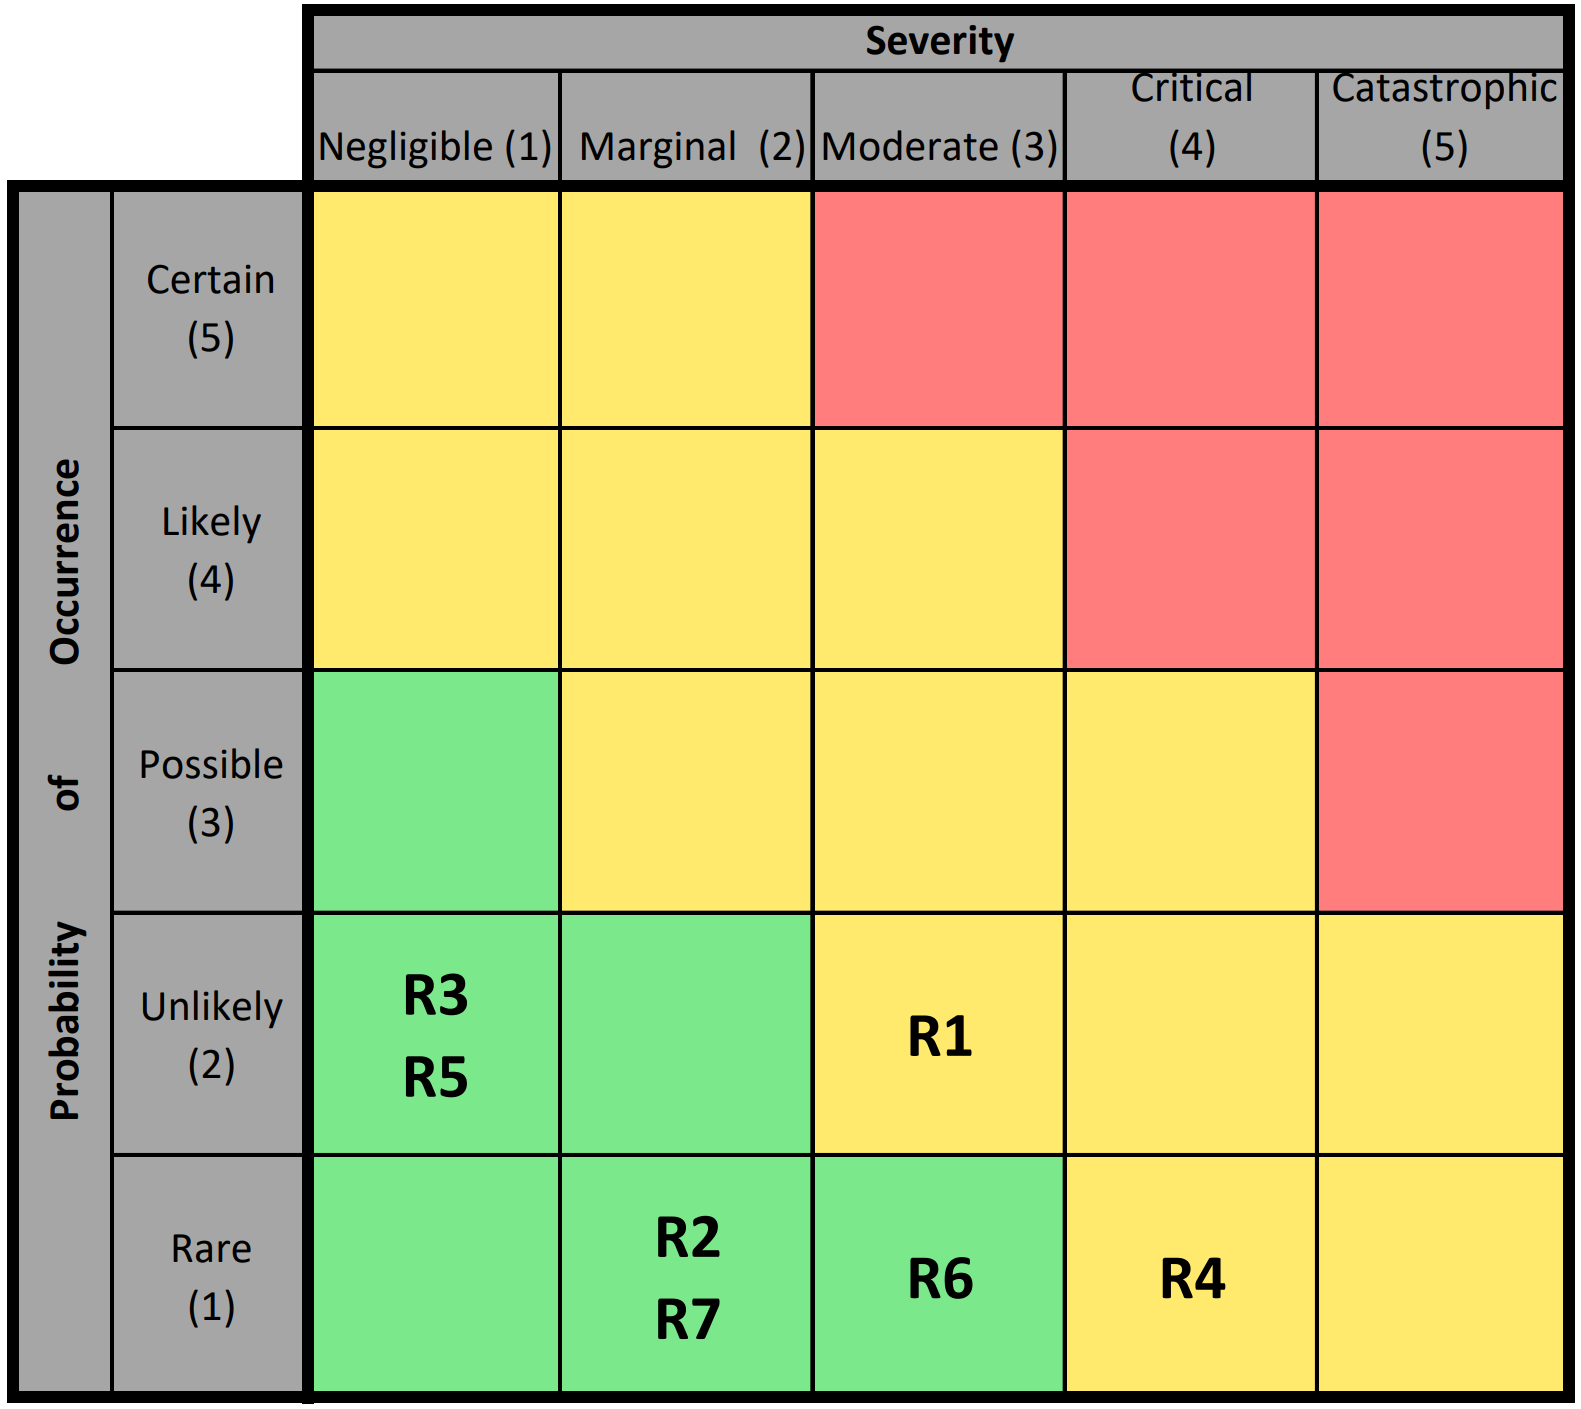
\includegraphics[width=0.6\textwidth]{resources/RiskMatrix.PNG}
    \caption{Risk Matrix}
    \label{fig:riskMatrix}
\end{figure}

\subsection{Mitigations}

In case one or more of the listed risks arise and turn into issues,
there are mitigations in place in order to reduce the severity of these issues.
These mitigations are shown in \ref*{tab:mitigations}.

\begin{table}[!ht]
    \makebox[\textwidth][c]{
        \begin{tabular}{ p{2cm} p{12.15cm}}
            \textbf{Risk Nr.} & \textbf{Mitigation} \\ \hline \\                                                                                                                                                                           
            \textbf{R1} & The people who worked on the stepper previously can be consulted in case there are any problems with existing software. \\
            \textbf{R2} & A time buffer at the end of the project is set in place, in case of sickness. \\
            \textbf{R3} & A time buffer at the end of the project is set in place, in case the estimates are too low. \\
            \textbf{R4} & A proof of concept is done at the start of the project. If it doesn't meet the requirements, a switch to a GUI could be done. \\
            \textbf{R5} & The GUI tool is not an essential feature and can thus be omitted. \\
            \textbf{R6} & Definition of an NFR that keeps the usage as simple as possible. \\
            \textbf{R7} & A time buffer at the end of the project is set in place, in case some functionality needs to be added in the core stepper. \\
        \end{tabular}
    }
    \caption{Mitigations for the identified risks.}
    \label{tab:mitigations}
\end{table}

\subsection{Arisen Issues}
During the project,
some of the risks that were identified during the planning of the project became issues.

\subsubsection*{R1}
It took me a while to get familiar with Core and to understand what was going on and how to understand the steps that are executed by the CoreStepper.
Luckily I could consider the developer of the CoreStepper for help and to understand what exactly was going on.
So while it took some time, it was not too much time that was spent on this.

\subsubsection*{R2}
While I got sick once,
that didn't affect the project too much,
as I was still able to put in work during that time.

\subsubsection*{Unforseen Risks}
Due to circumstances beyond my control,
an impactful incident in my private life kept me from working for about a week.
Thankfully, I was able to move the deadline of the project back by a week,
which mitigated this issue.

\chapter{Time Management}
This chapter shows the amount of time that went into the project.

\ \\
As can be seen in figure \ref*{fig:timeTracking},
the majority of the time was spent on improving the prototype.
Almost half of the time (178 hours) was spent on refactorings and usability upgrades.
This includes the manual and interactive modes, as well as highlighting text on the terminal and the user interaction overall.

\ \\
Creating the base prototype took around 111 hours,
which includes the research that had to be done about the Core language as well as some Haskell language features that would be used in the project.
The result was a prototype that could do step Haskell automatically but not manually.

\ \\
The documentation also took a good amount of time,
making up for over a sixth of the total time spent, spread over the three last weeks.

\ \\
Meetings with the advisor and other people that are involved in the project took less than 24 hours combined,
which comes to a bit over 1 hour per week.

\ \\
The time spent overall comes to around 383 hours, which equals a weekly workload of around 21 hours and 20 minutes.

\begin{figure}
    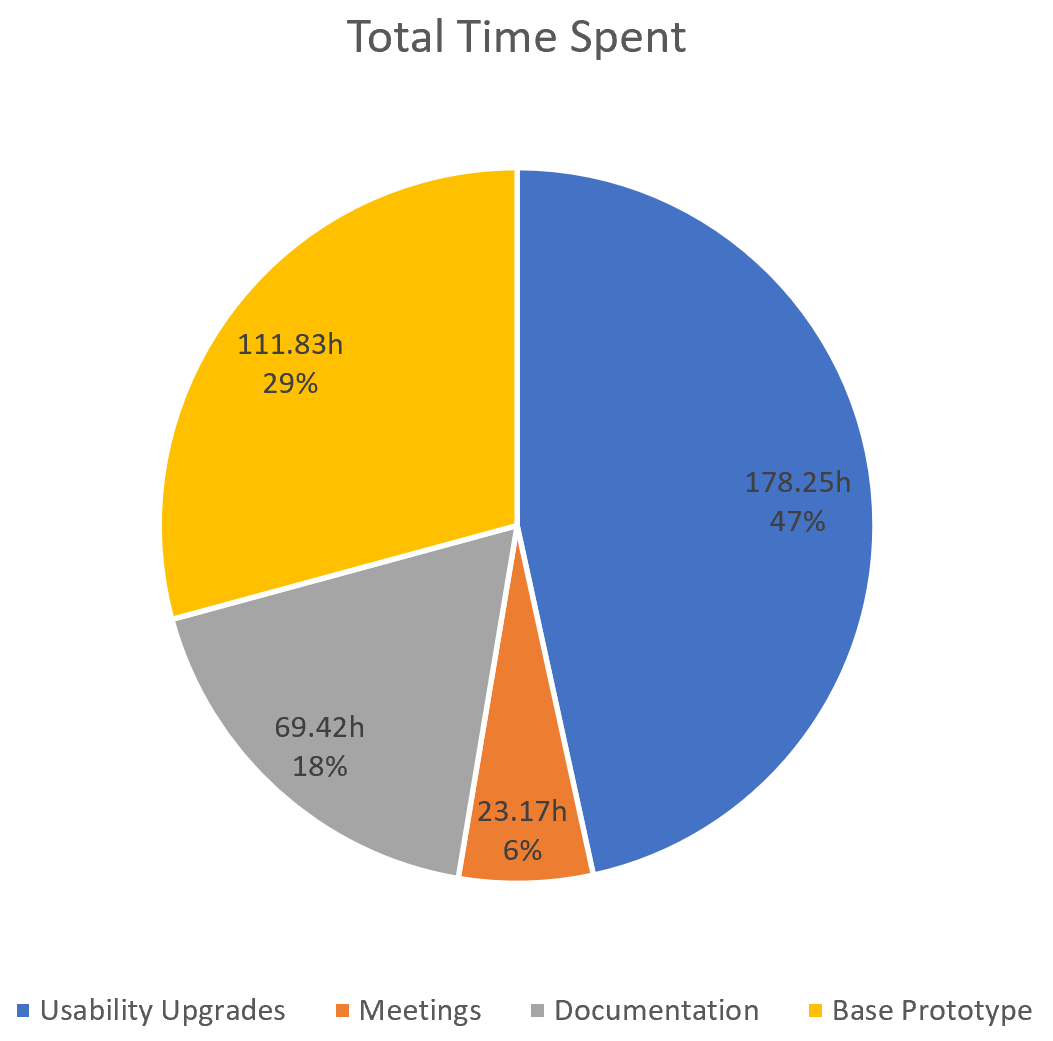
\includegraphics[width=1\textwidth]{resources/time_tracking.PNG}
    \caption{Time spent by epic}
    \label{fig:timeTracking}
\end{figure}

\chapter{Examples}
\label{chptr:examples}
This chapter contains some examples of how the Substitution Stepper steps some of the examples from the task description.
The derivations are somewhat long still compared to the examples given in the task description.

\section{Example 1}
The first example sums up three elements in a list.
Due to the limitations of the stepper,
the Nat datatype was used instead of Int.

\begin{figure}
    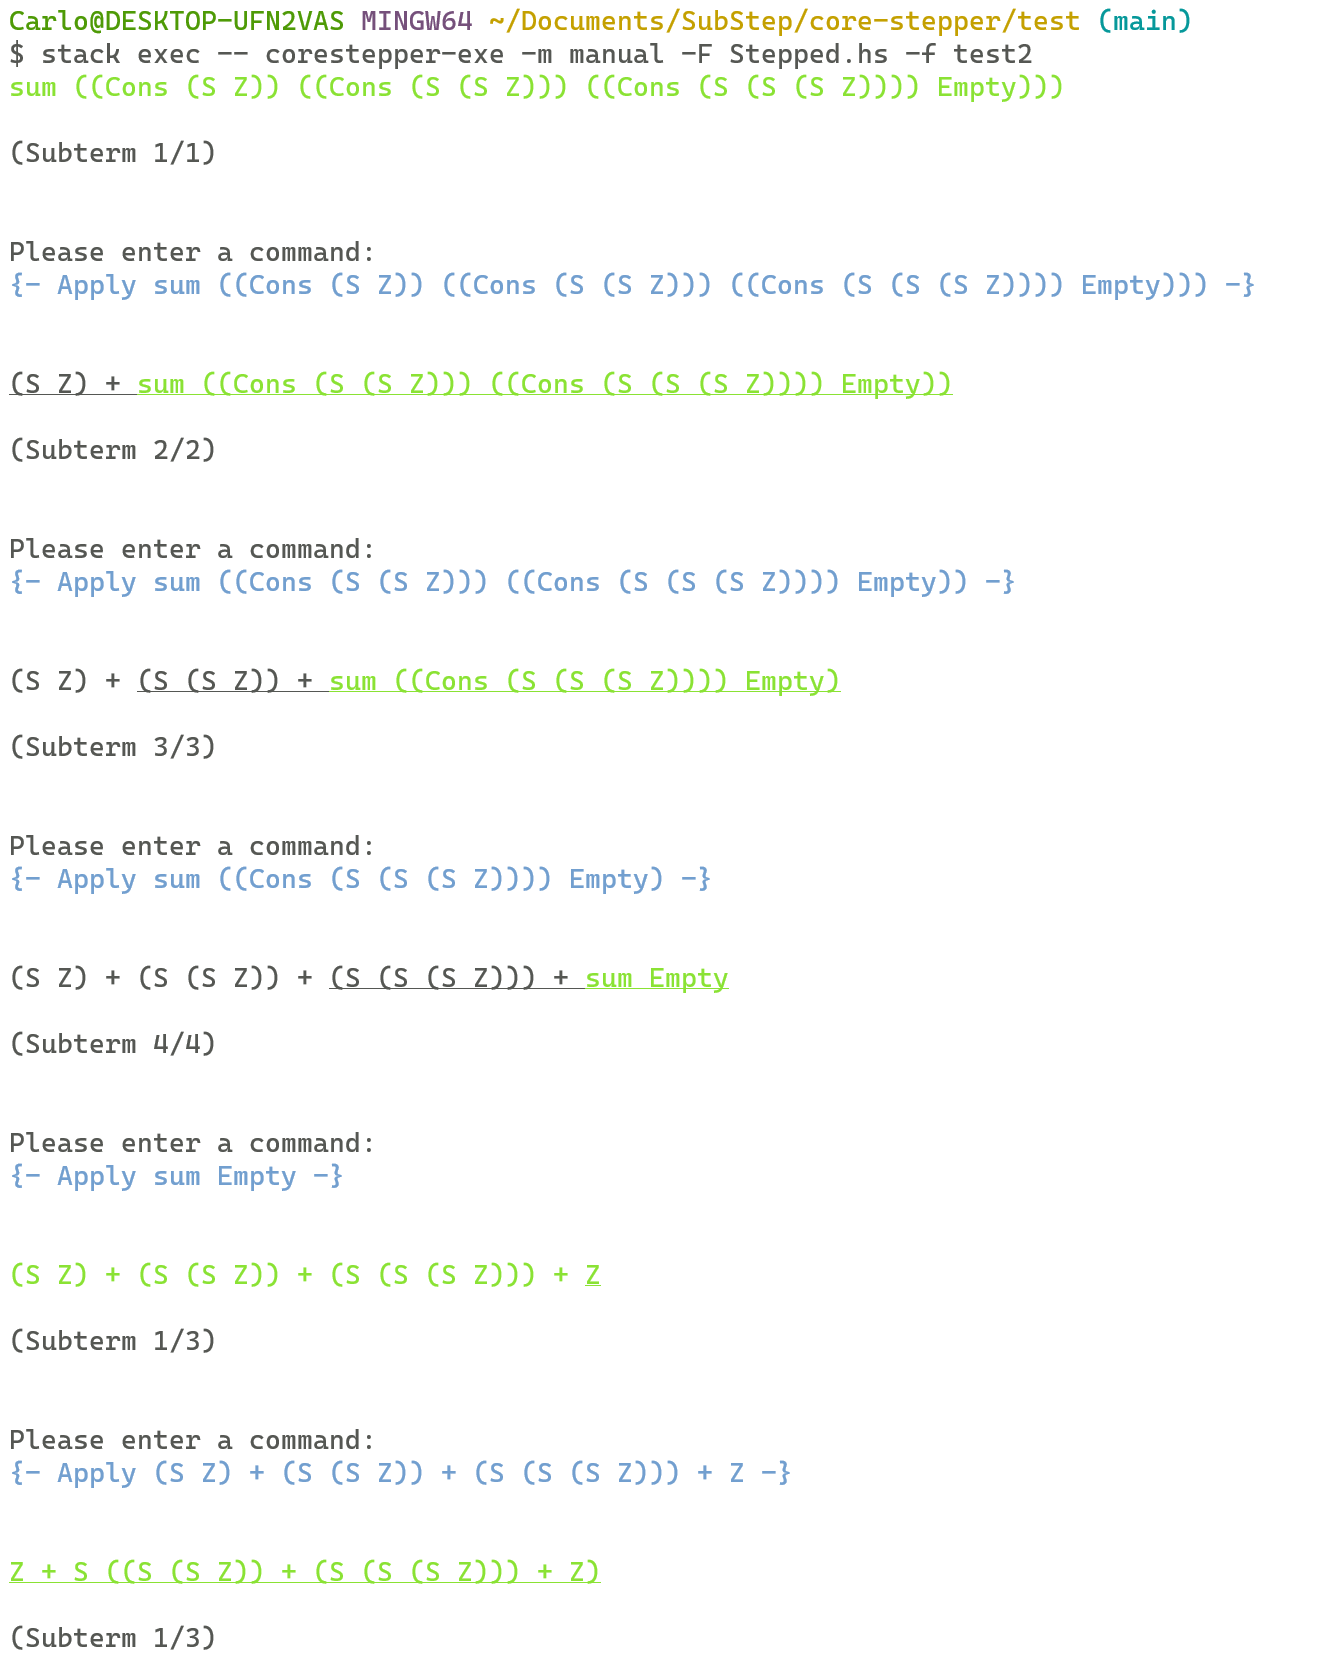
\includegraphics[width=1\textwidth]{resources/sum_part_1.PNG}
\end{figure}
\begin{figure}
    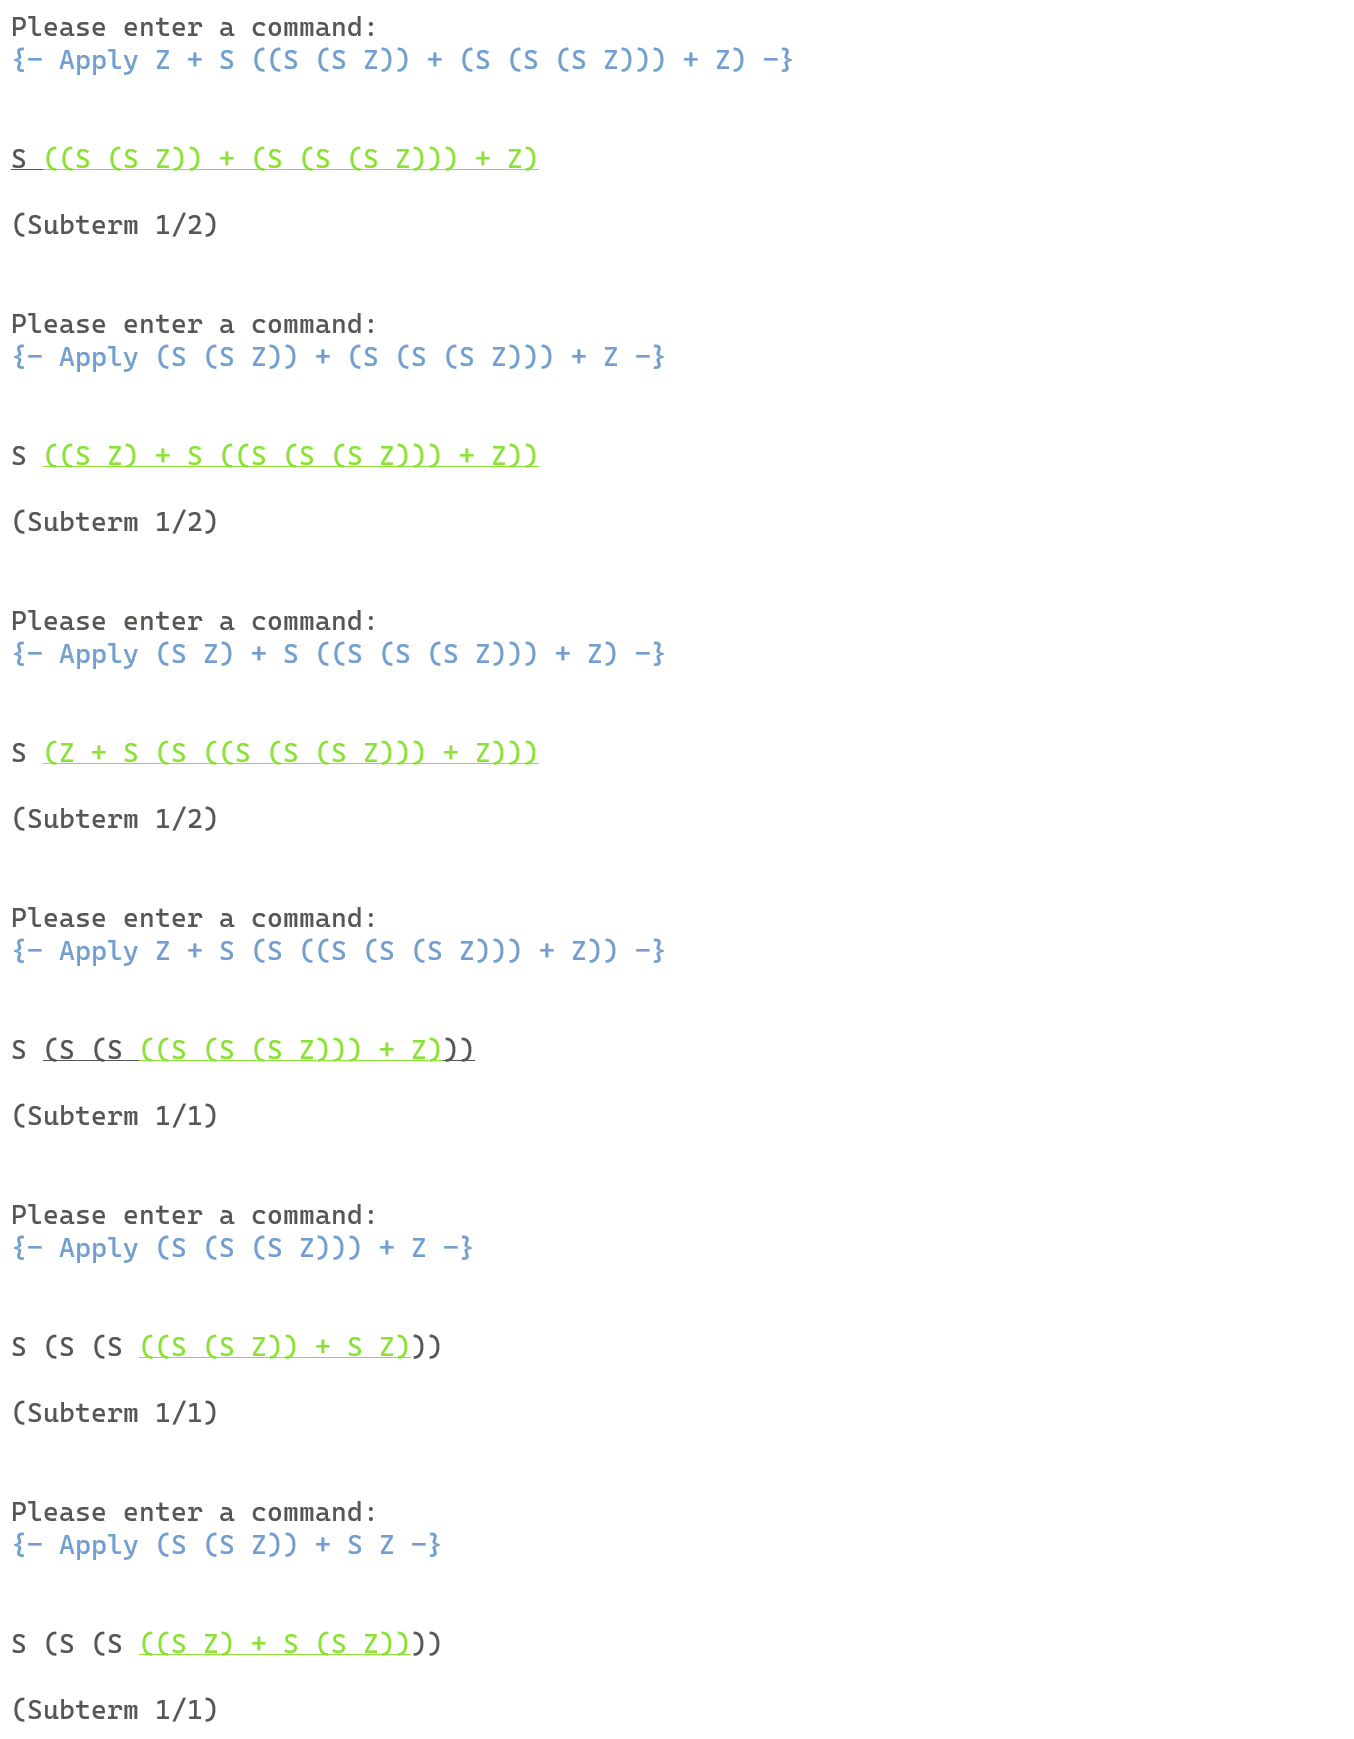
\includegraphics[width=1\textwidth]{resources/sum_part_2.PNG}
\end{figure}
\begin{figure}
    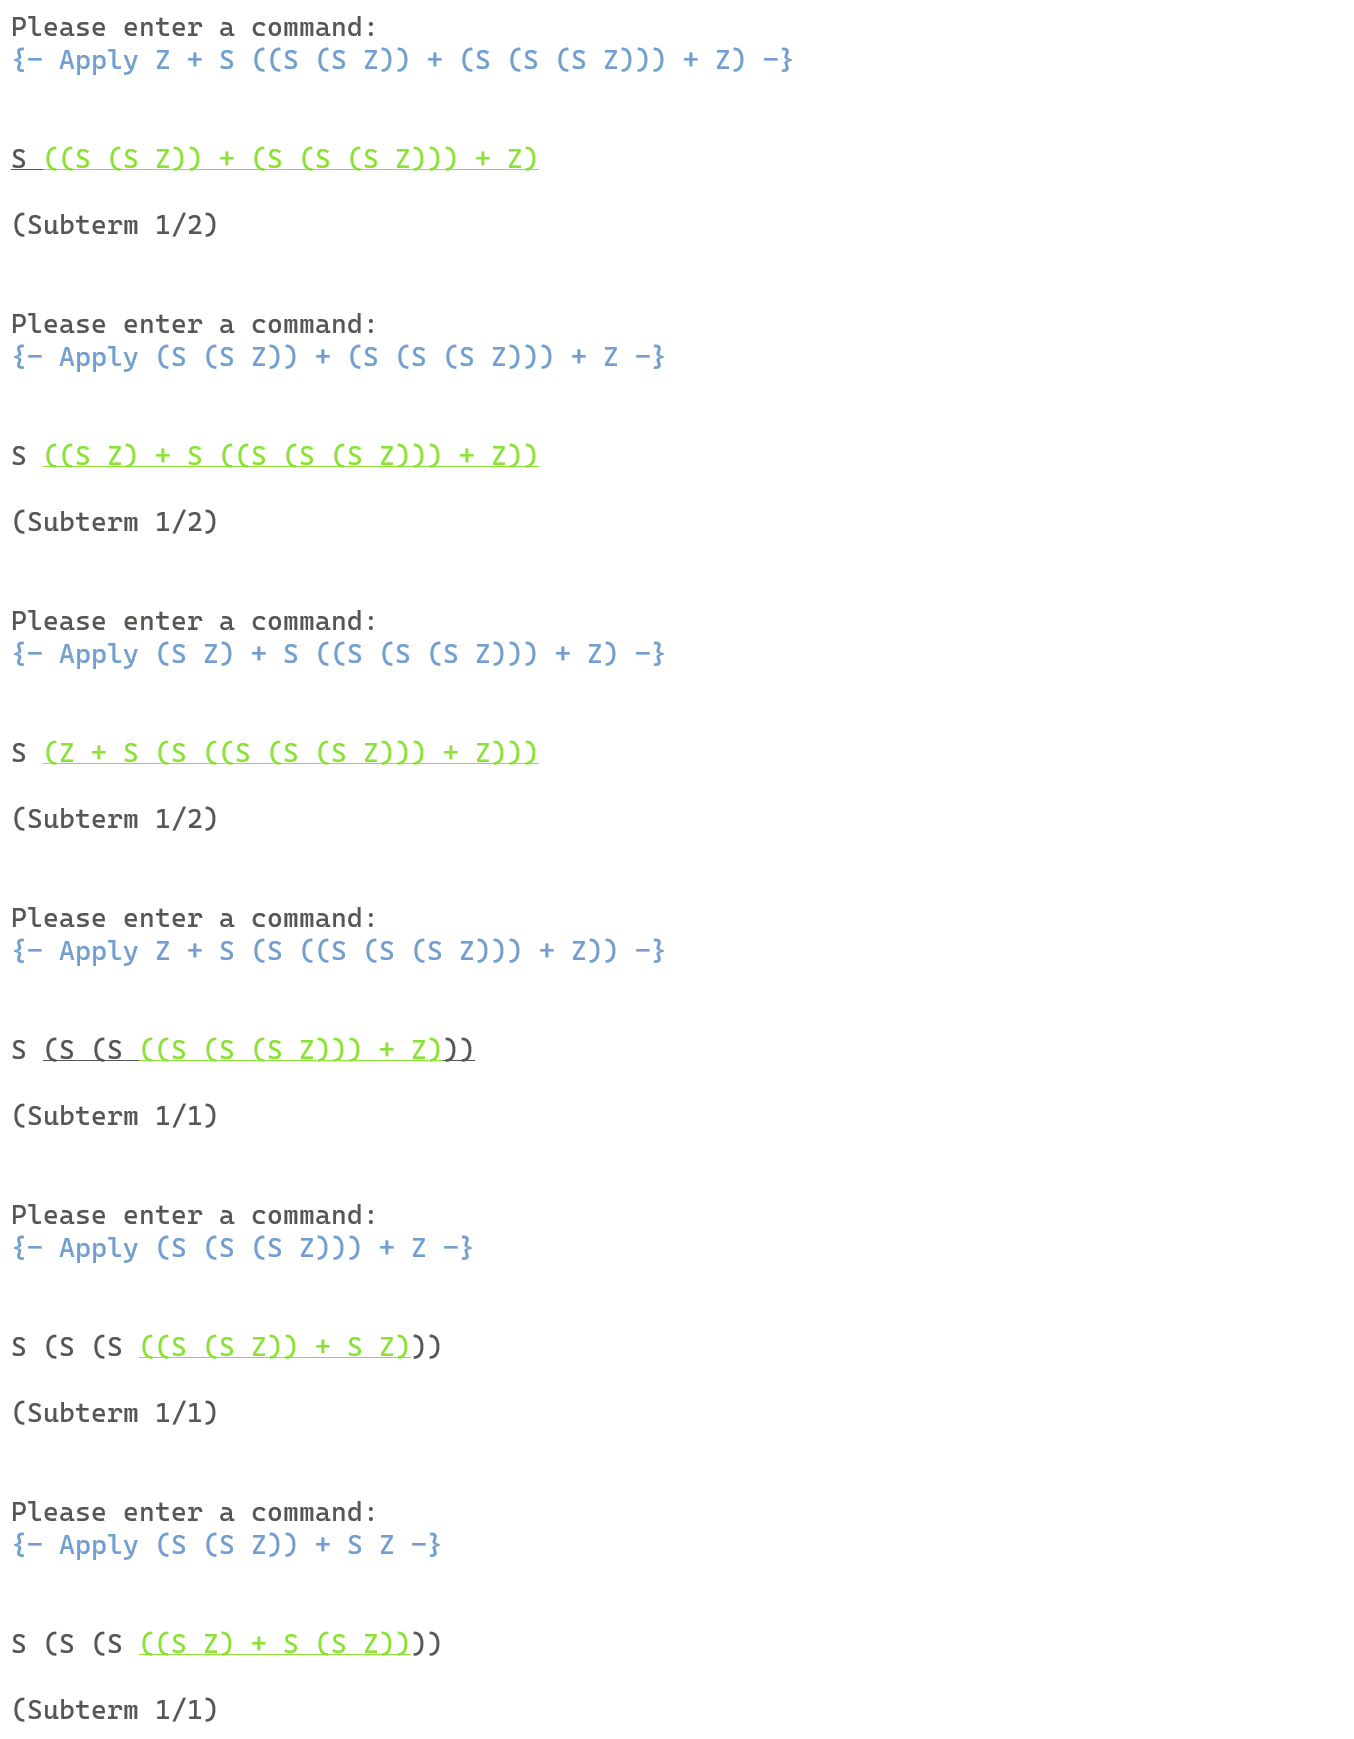
\includegraphics[width=1\textwidth]{resources/sum_part_2.PNG}
    \caption{The first example, summing 1, 2, and 3 in a list to obtain the value 6.}
\end{figure}

\clearpage
\section{Example 2}
The second example reverses a list containing 3 elements.
Again, this example had to be adjusted, this time it uses letters as they are more easily readable than the Nat datatype.

\begin{figure}
    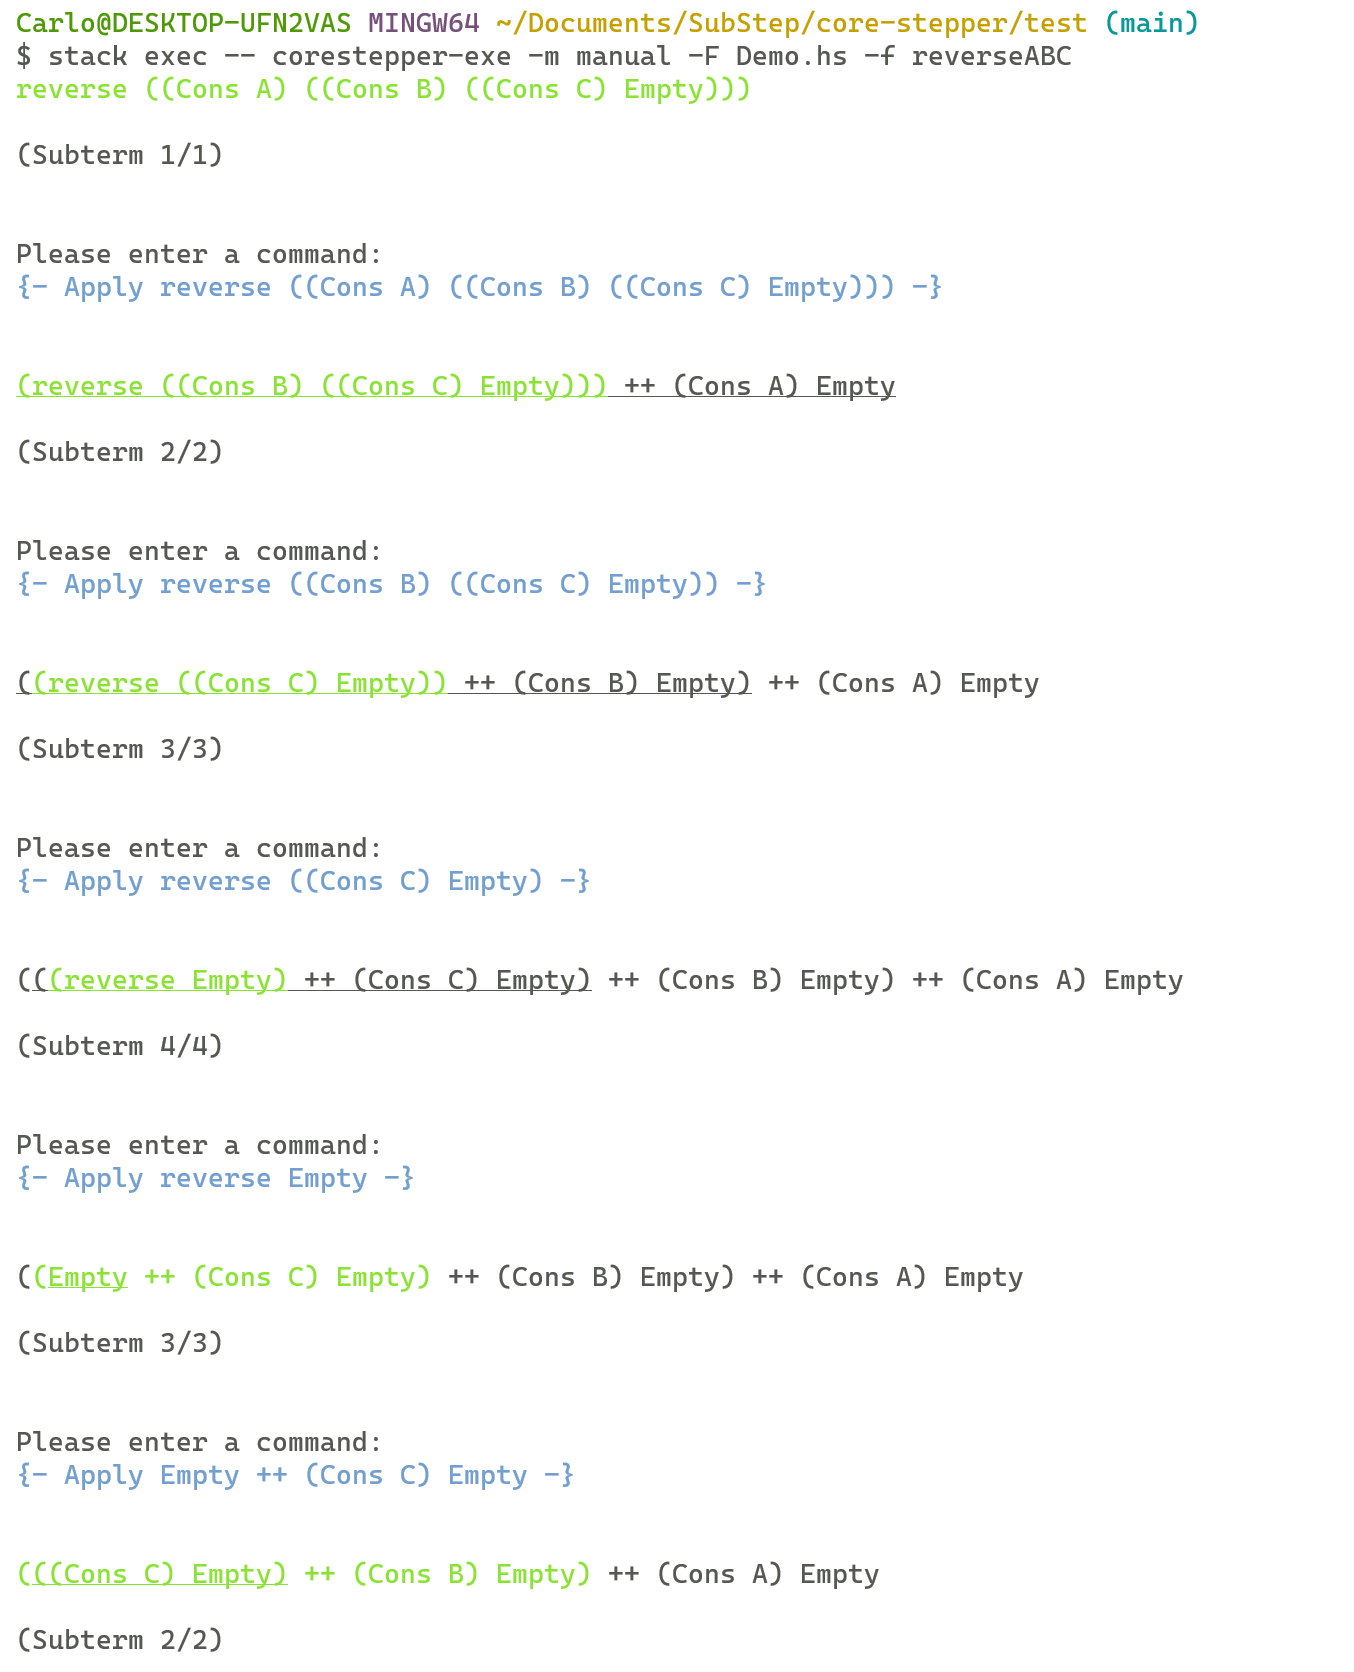
\includegraphics[width=1\textwidth]{resources/reverse_part_1.PNG}
\end{figure}
\begin{figure}
    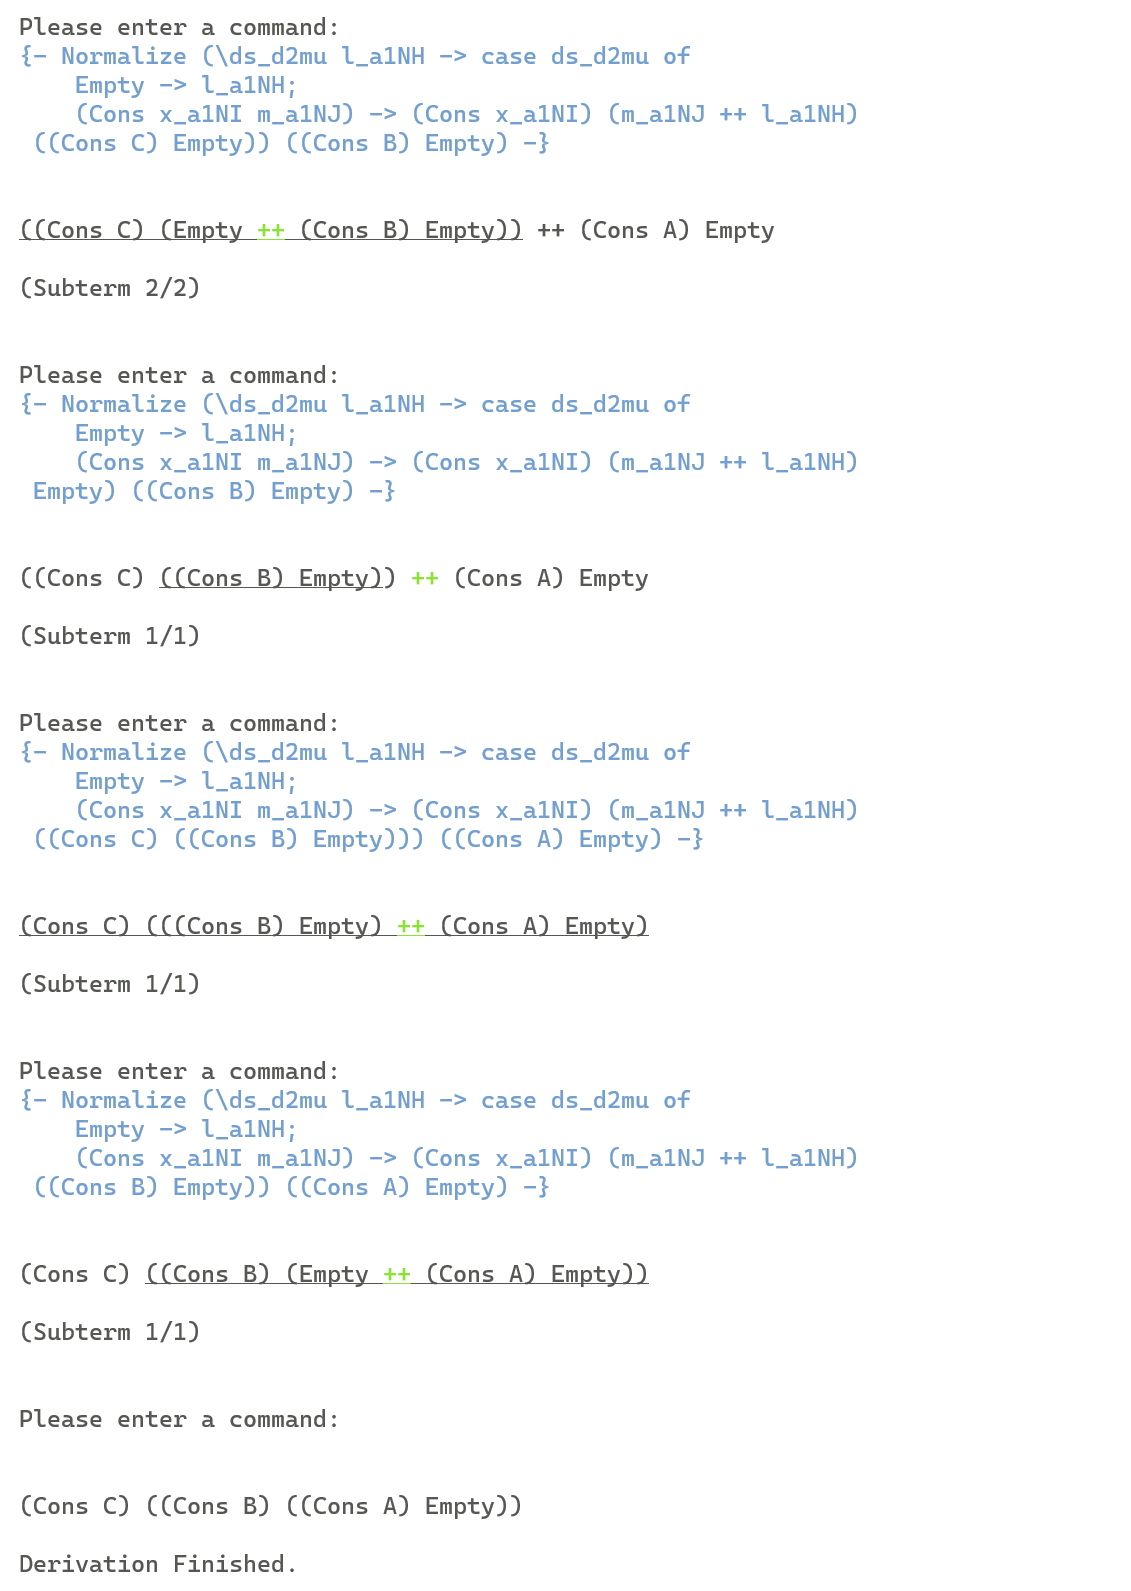
\includegraphics[width=1\textwidth]{resources/reverse_part_2.PNG}
    \caption{The second example, reversing the list [A,B,C].}
\end{figure}

\clearpage
\section{Example 3}
The third example uses the Nat datatype again.
It corresponds to \texttt{pure (+) <*> [1,2] <*> [3,4]}

\begin{figure}
    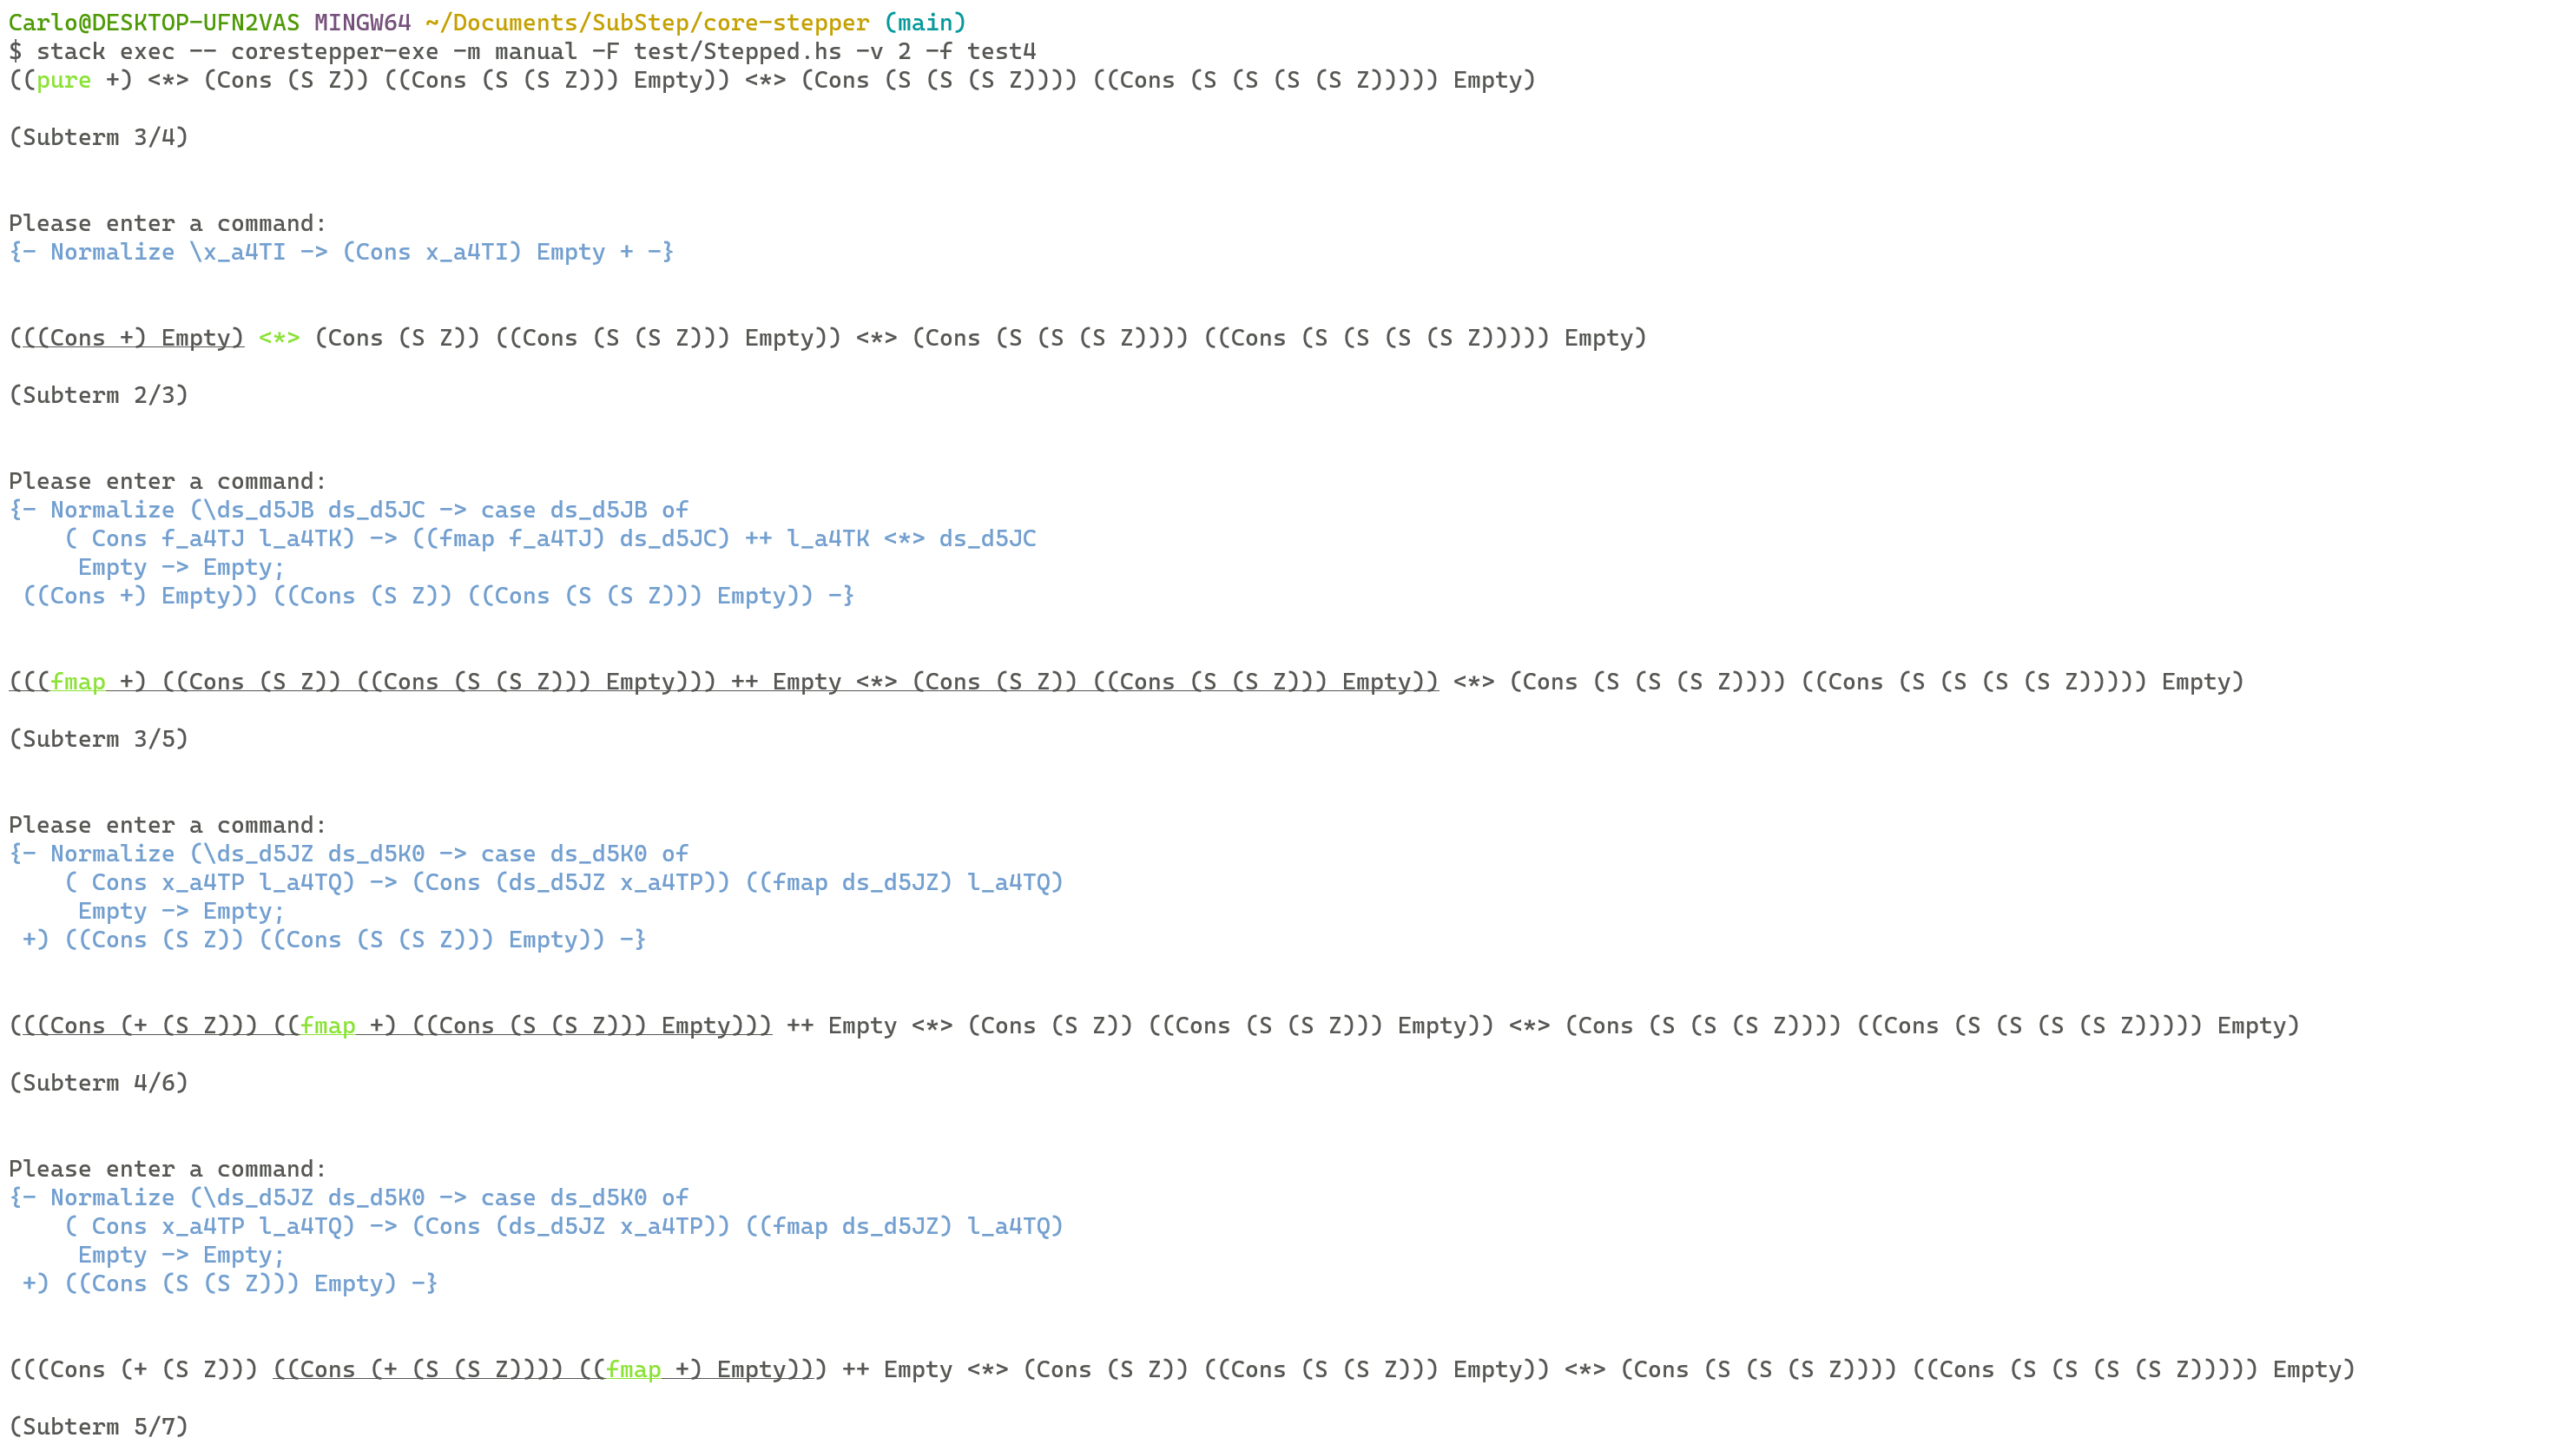
\includegraphics[width=1\textwidth]{resources/applicative_part_1.PNG}
\end{figure}
\begin{figure}
    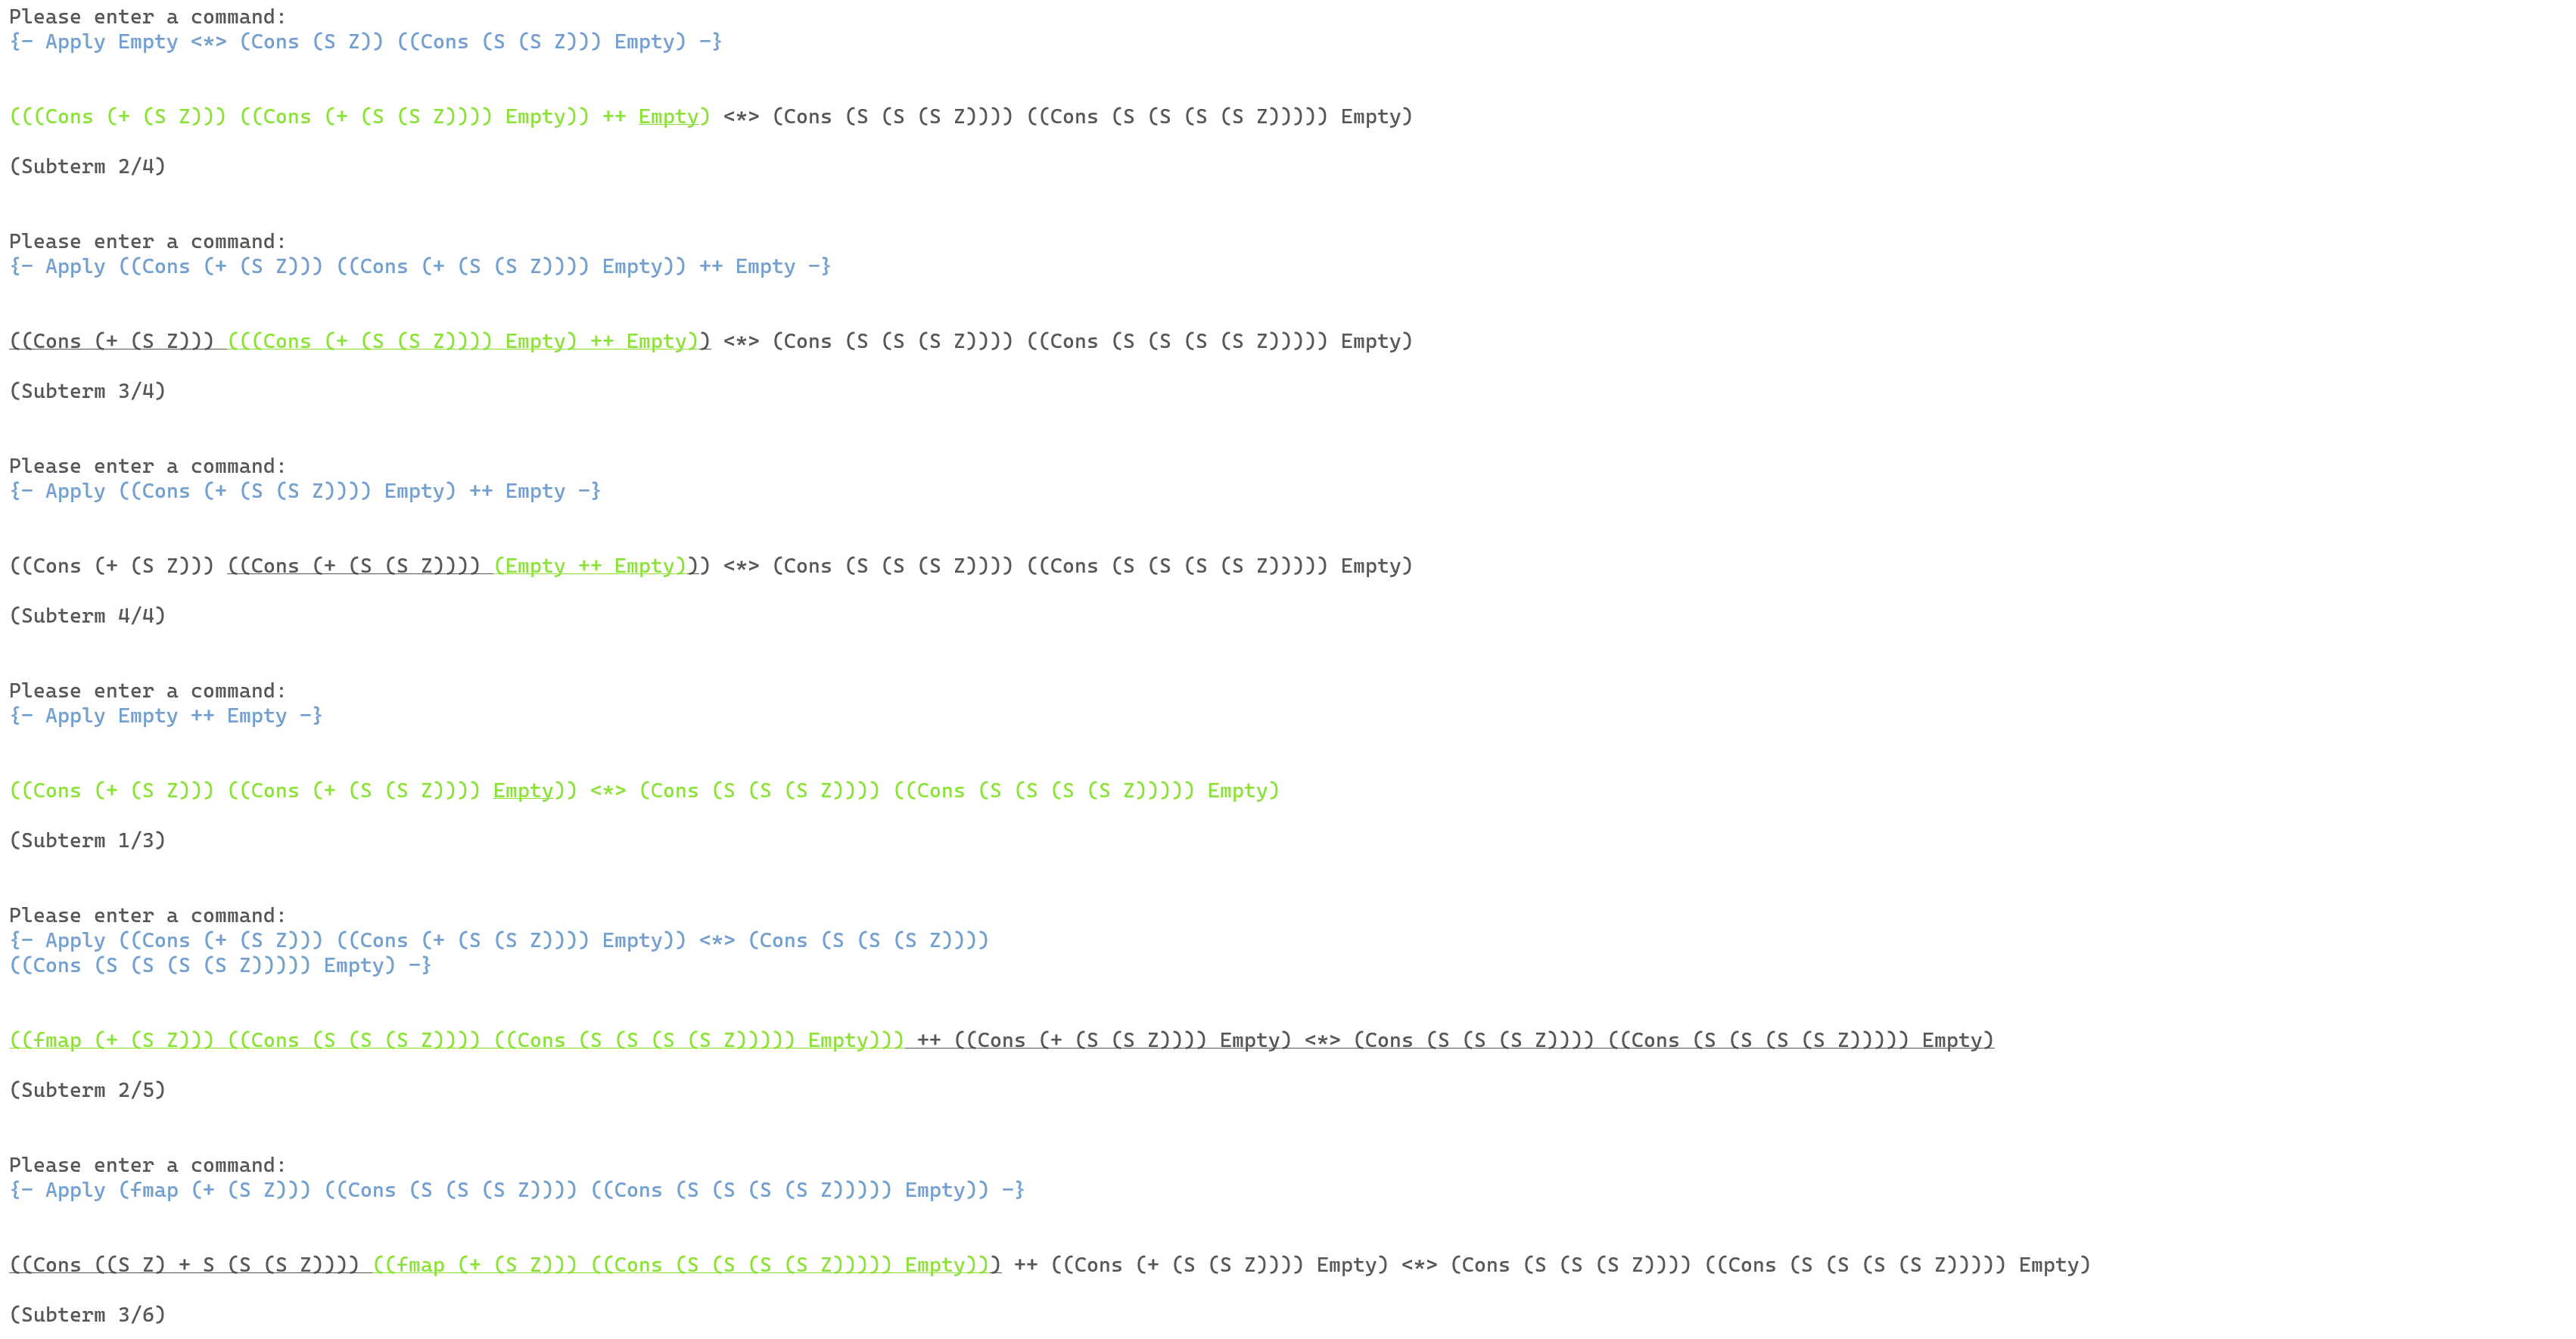
\includegraphics[width=1\textwidth]{resources/applicative_part_2.PNG}
\end{figure}
\begin{figure}
    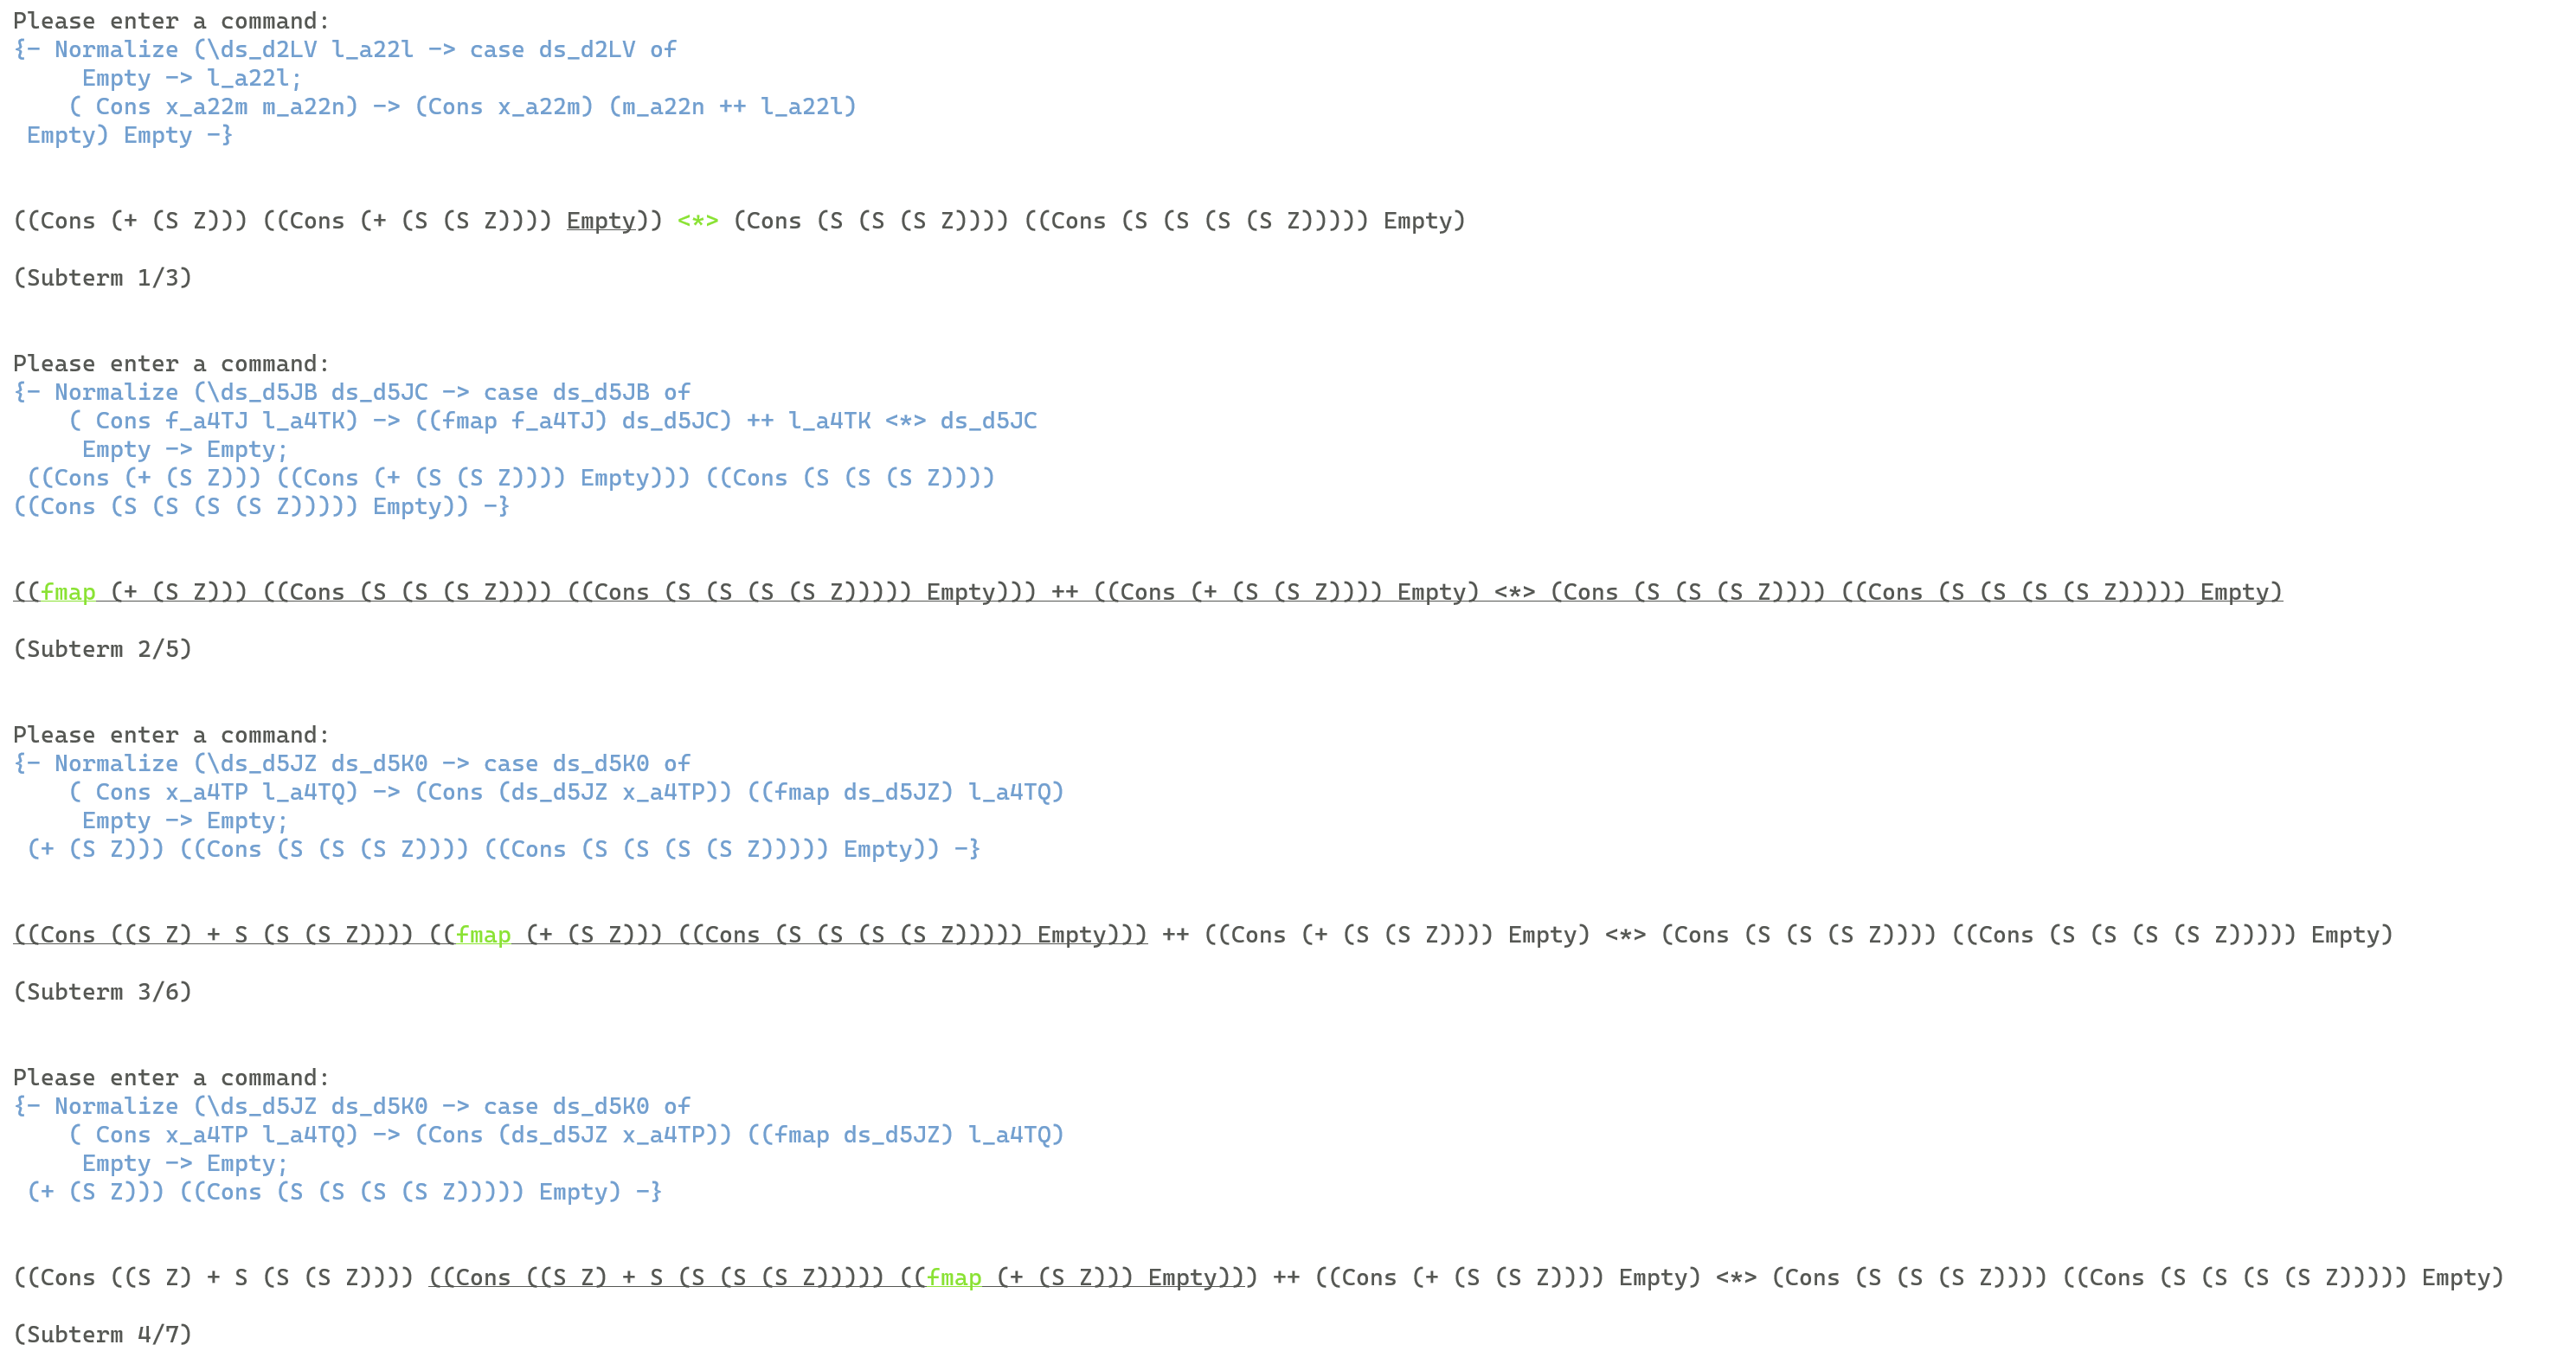
\includegraphics[width=1\textwidth]{resources/applicative_part_3.PNG}
\end{figure}
\begin{figure}
    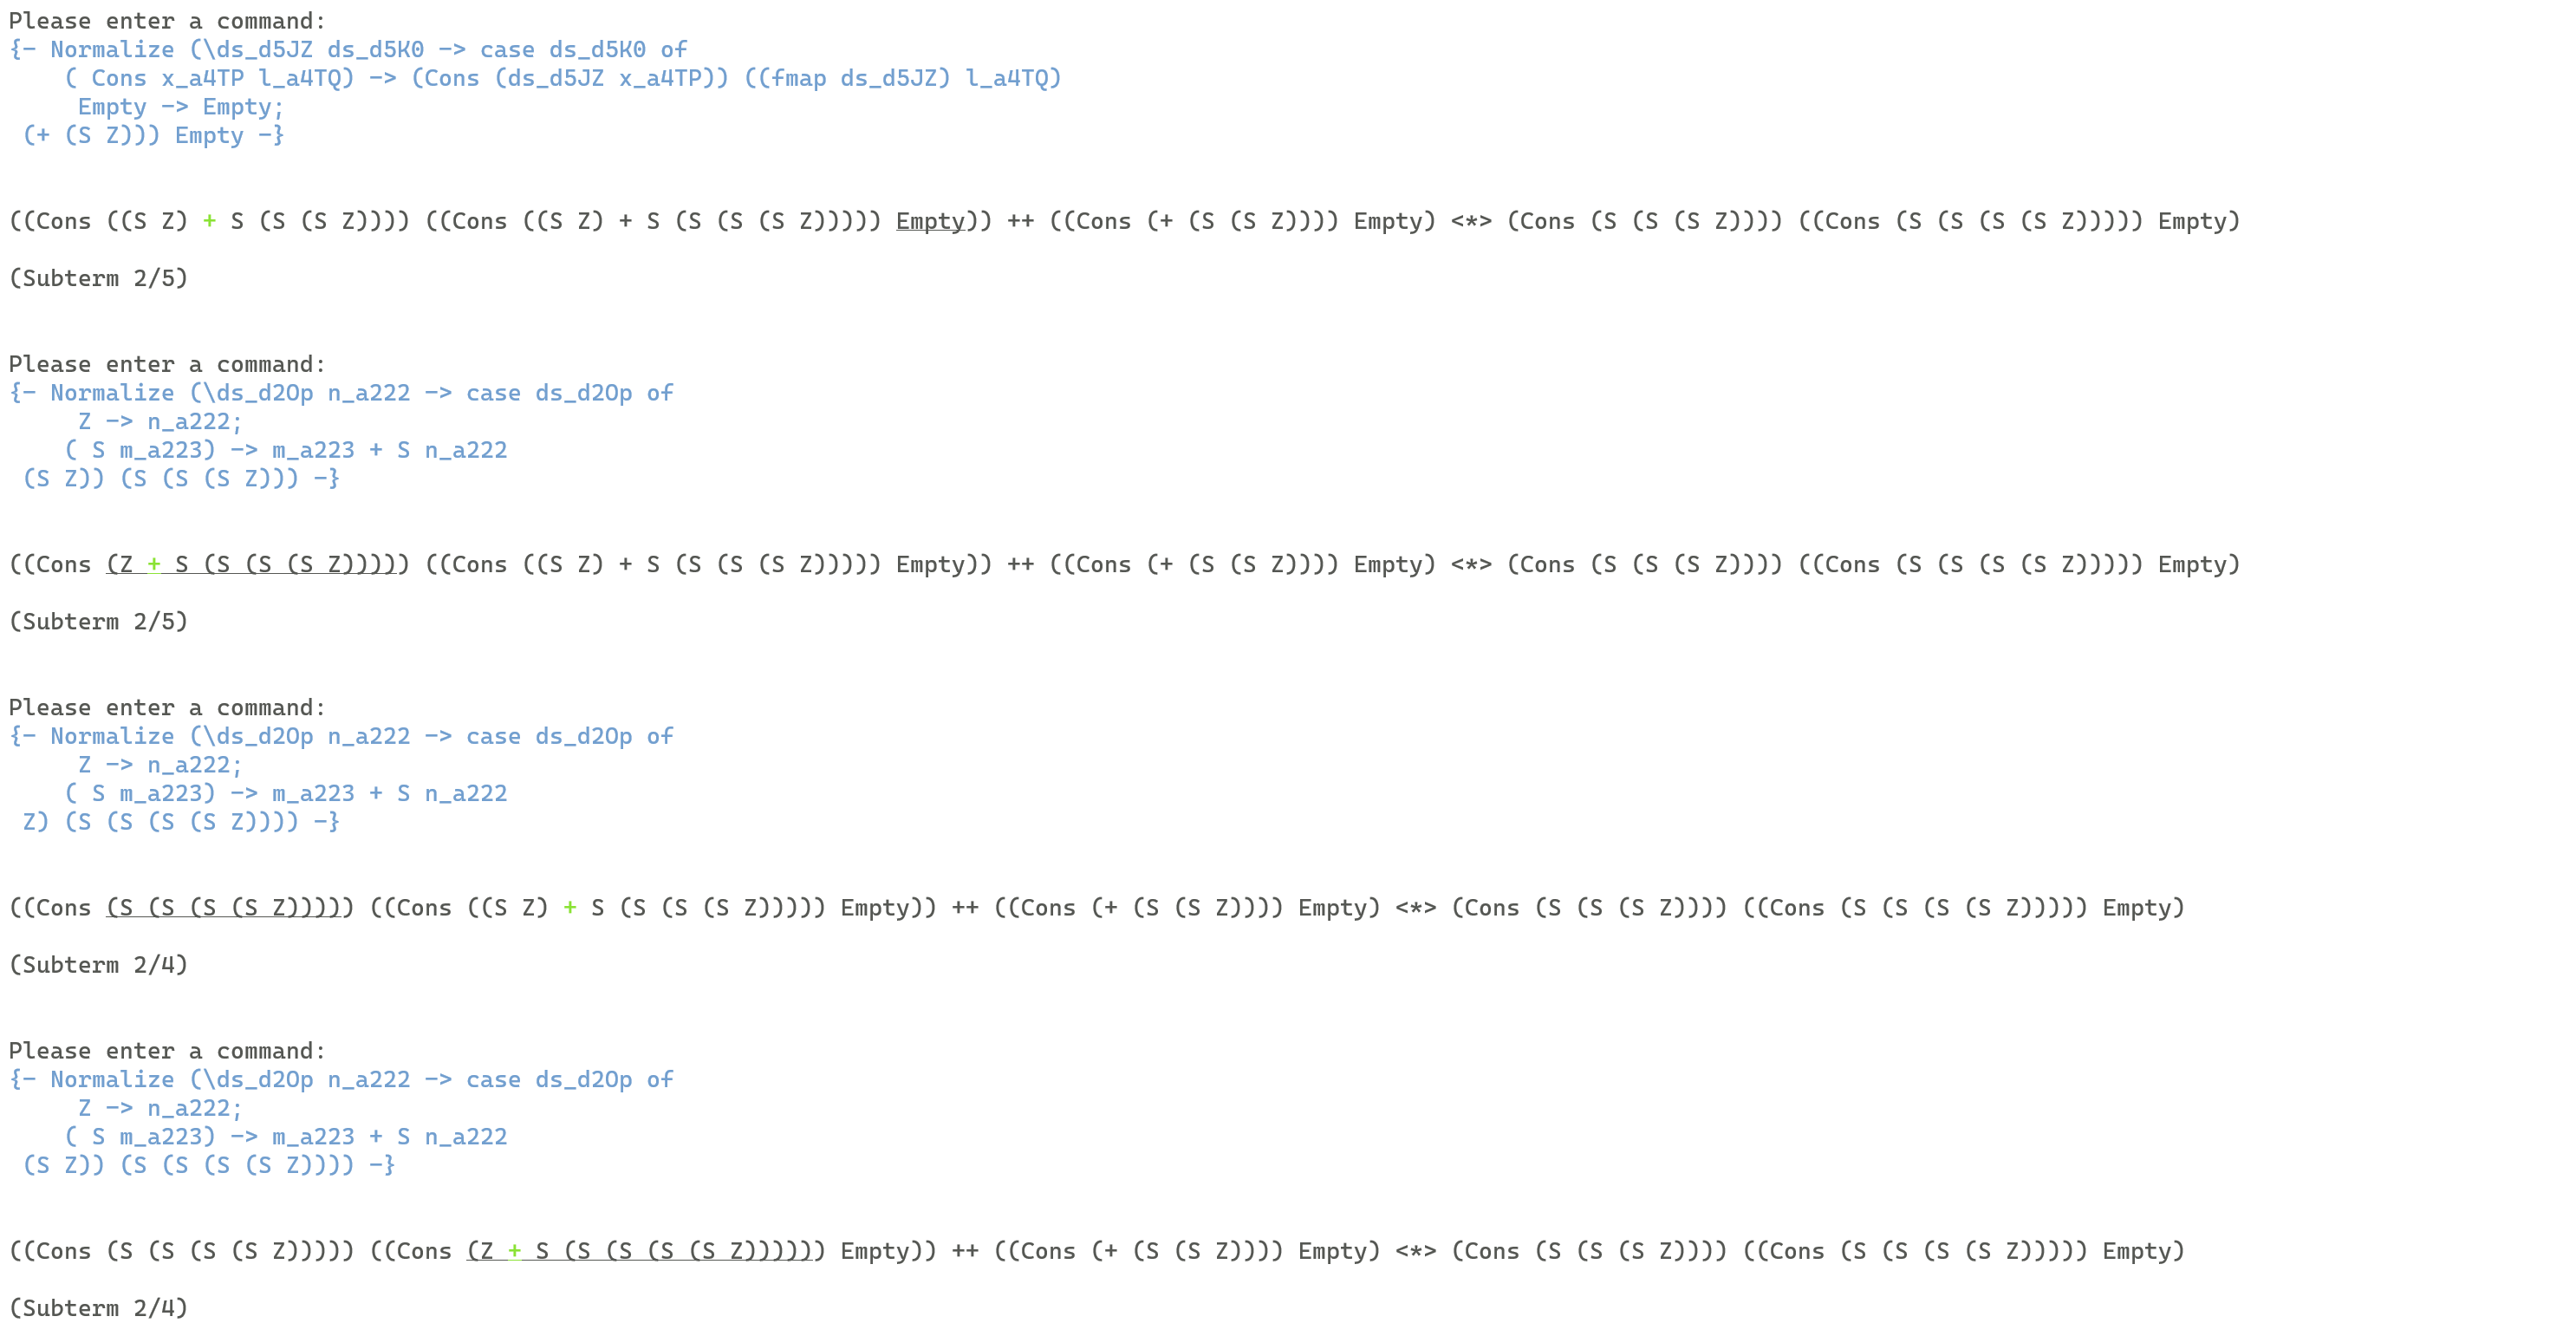
\includegraphics[width=1\textwidth]{resources/applicative_part_4.PNG}
\end{figure}
\begin{figure}
    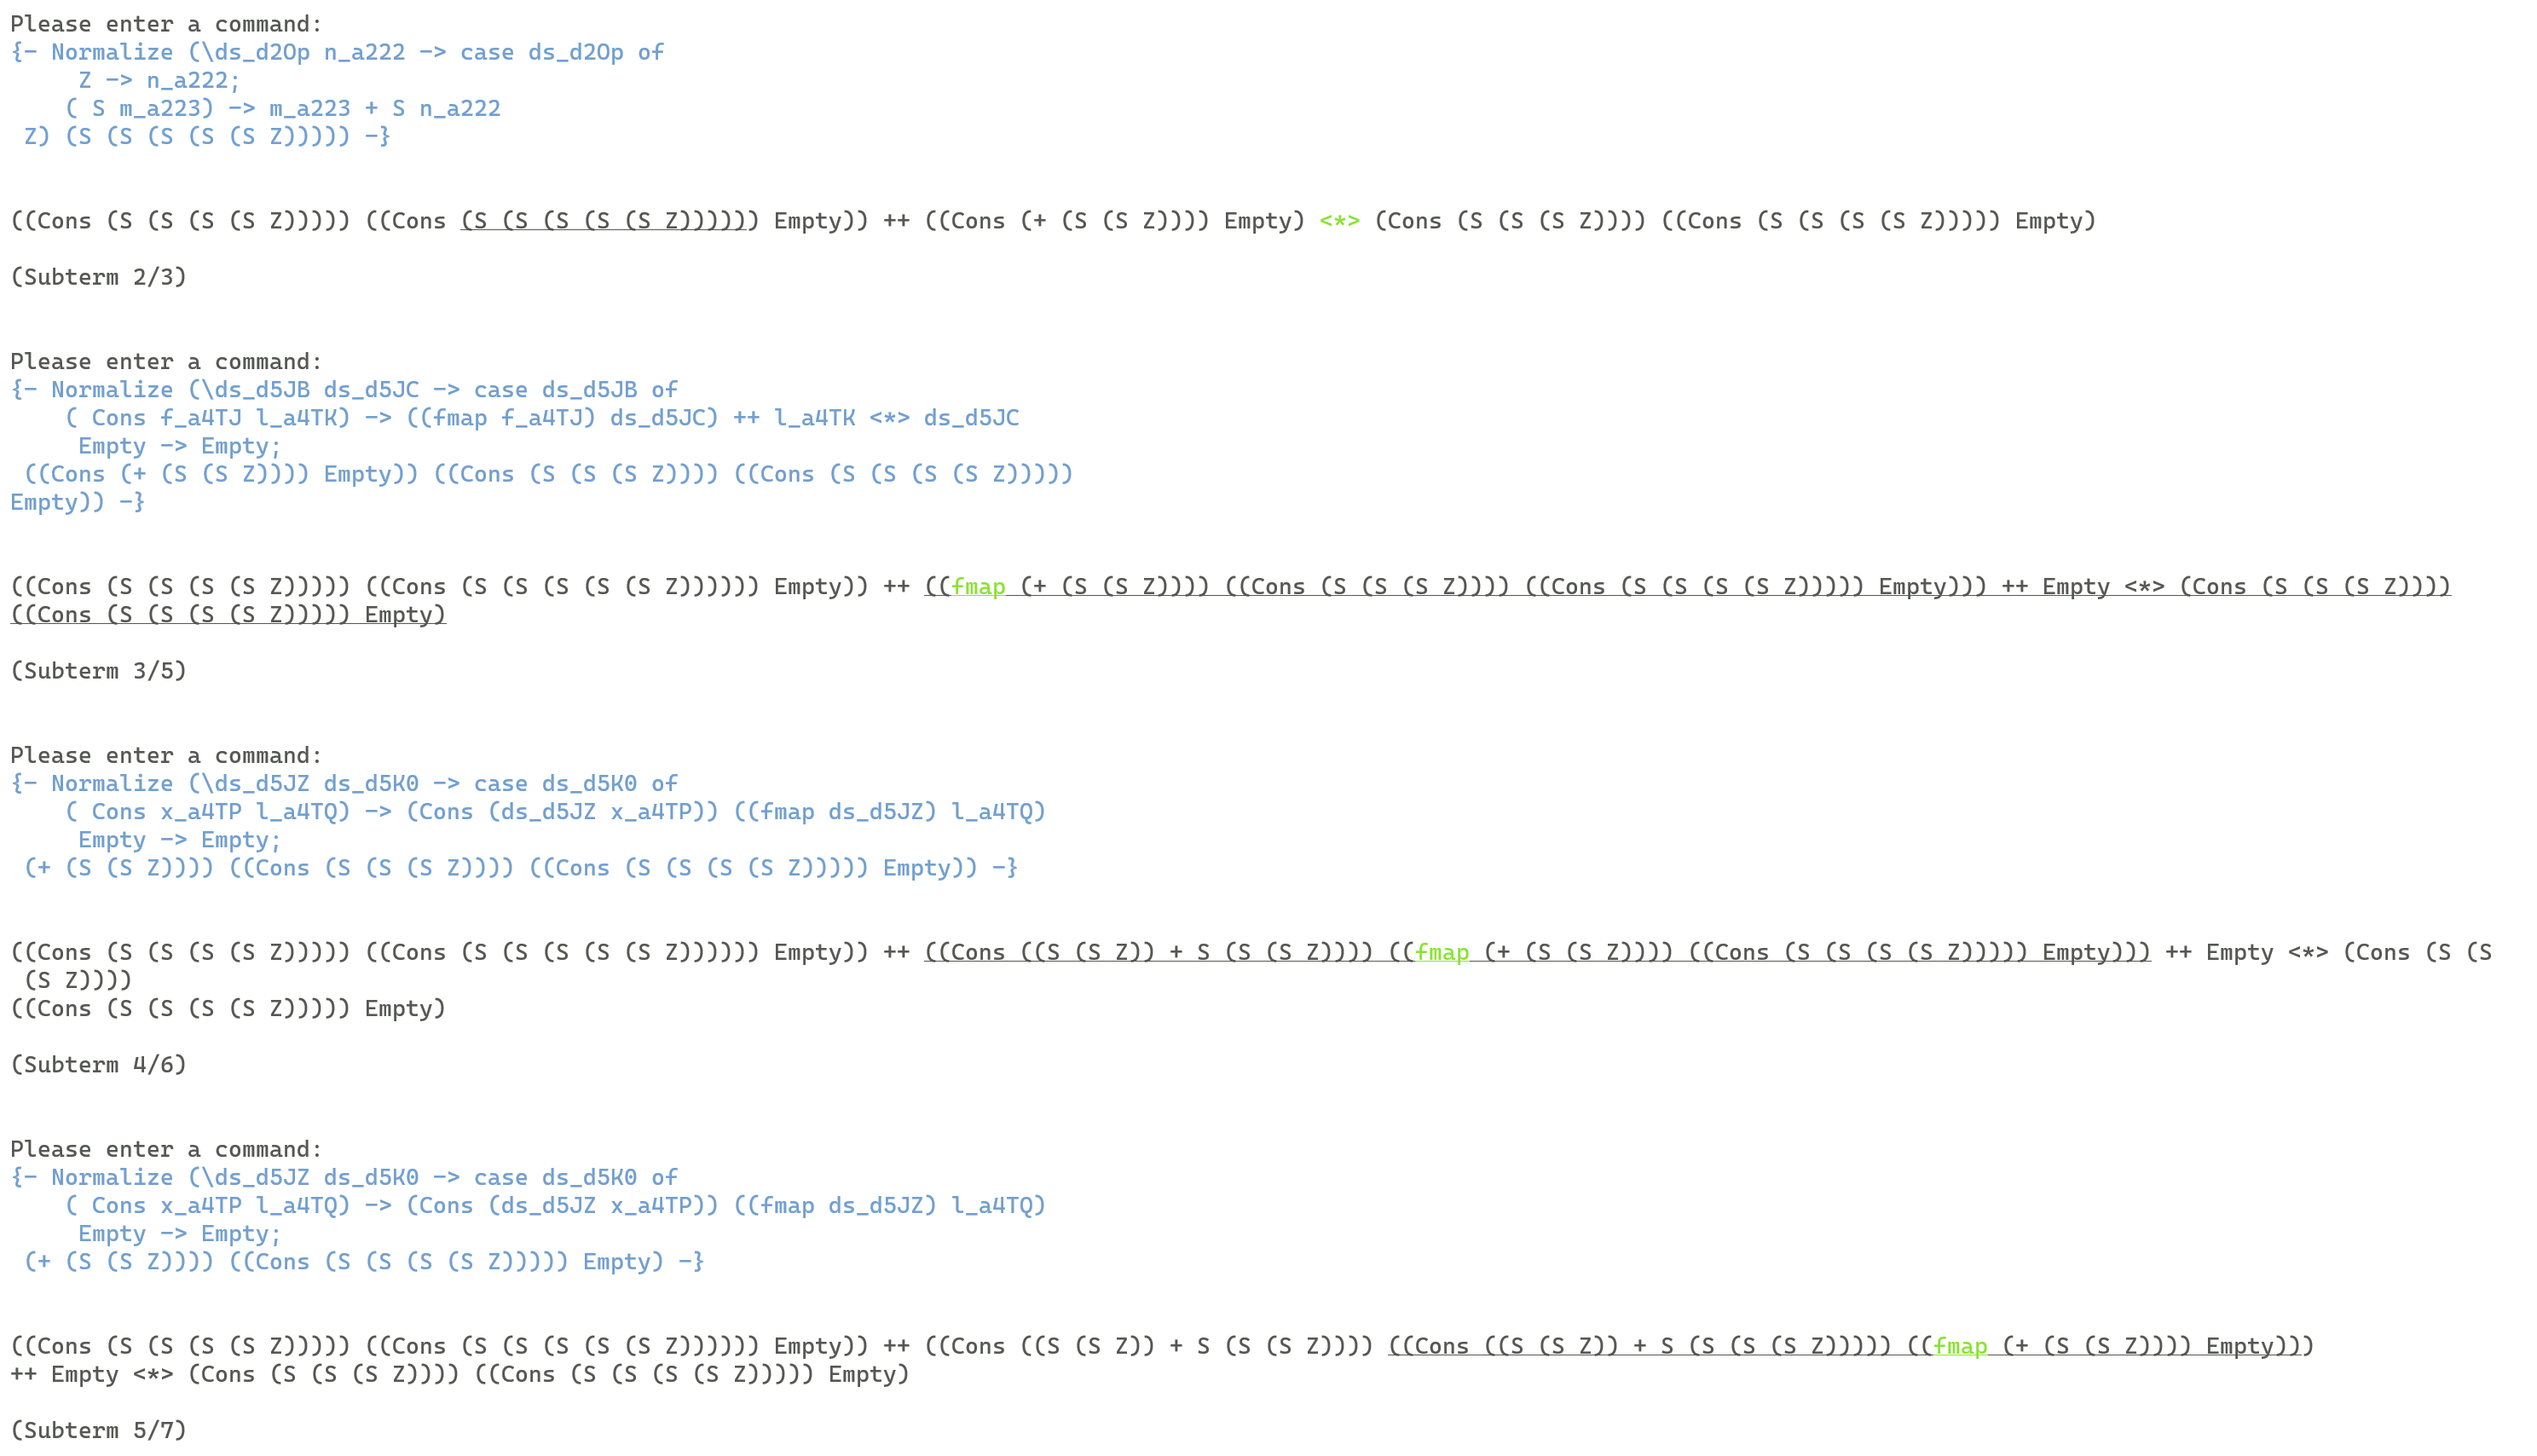
\includegraphics[width=1\textwidth]{resources/applicative_part_5.PNG}
\end{figure}
\begin{figure}
    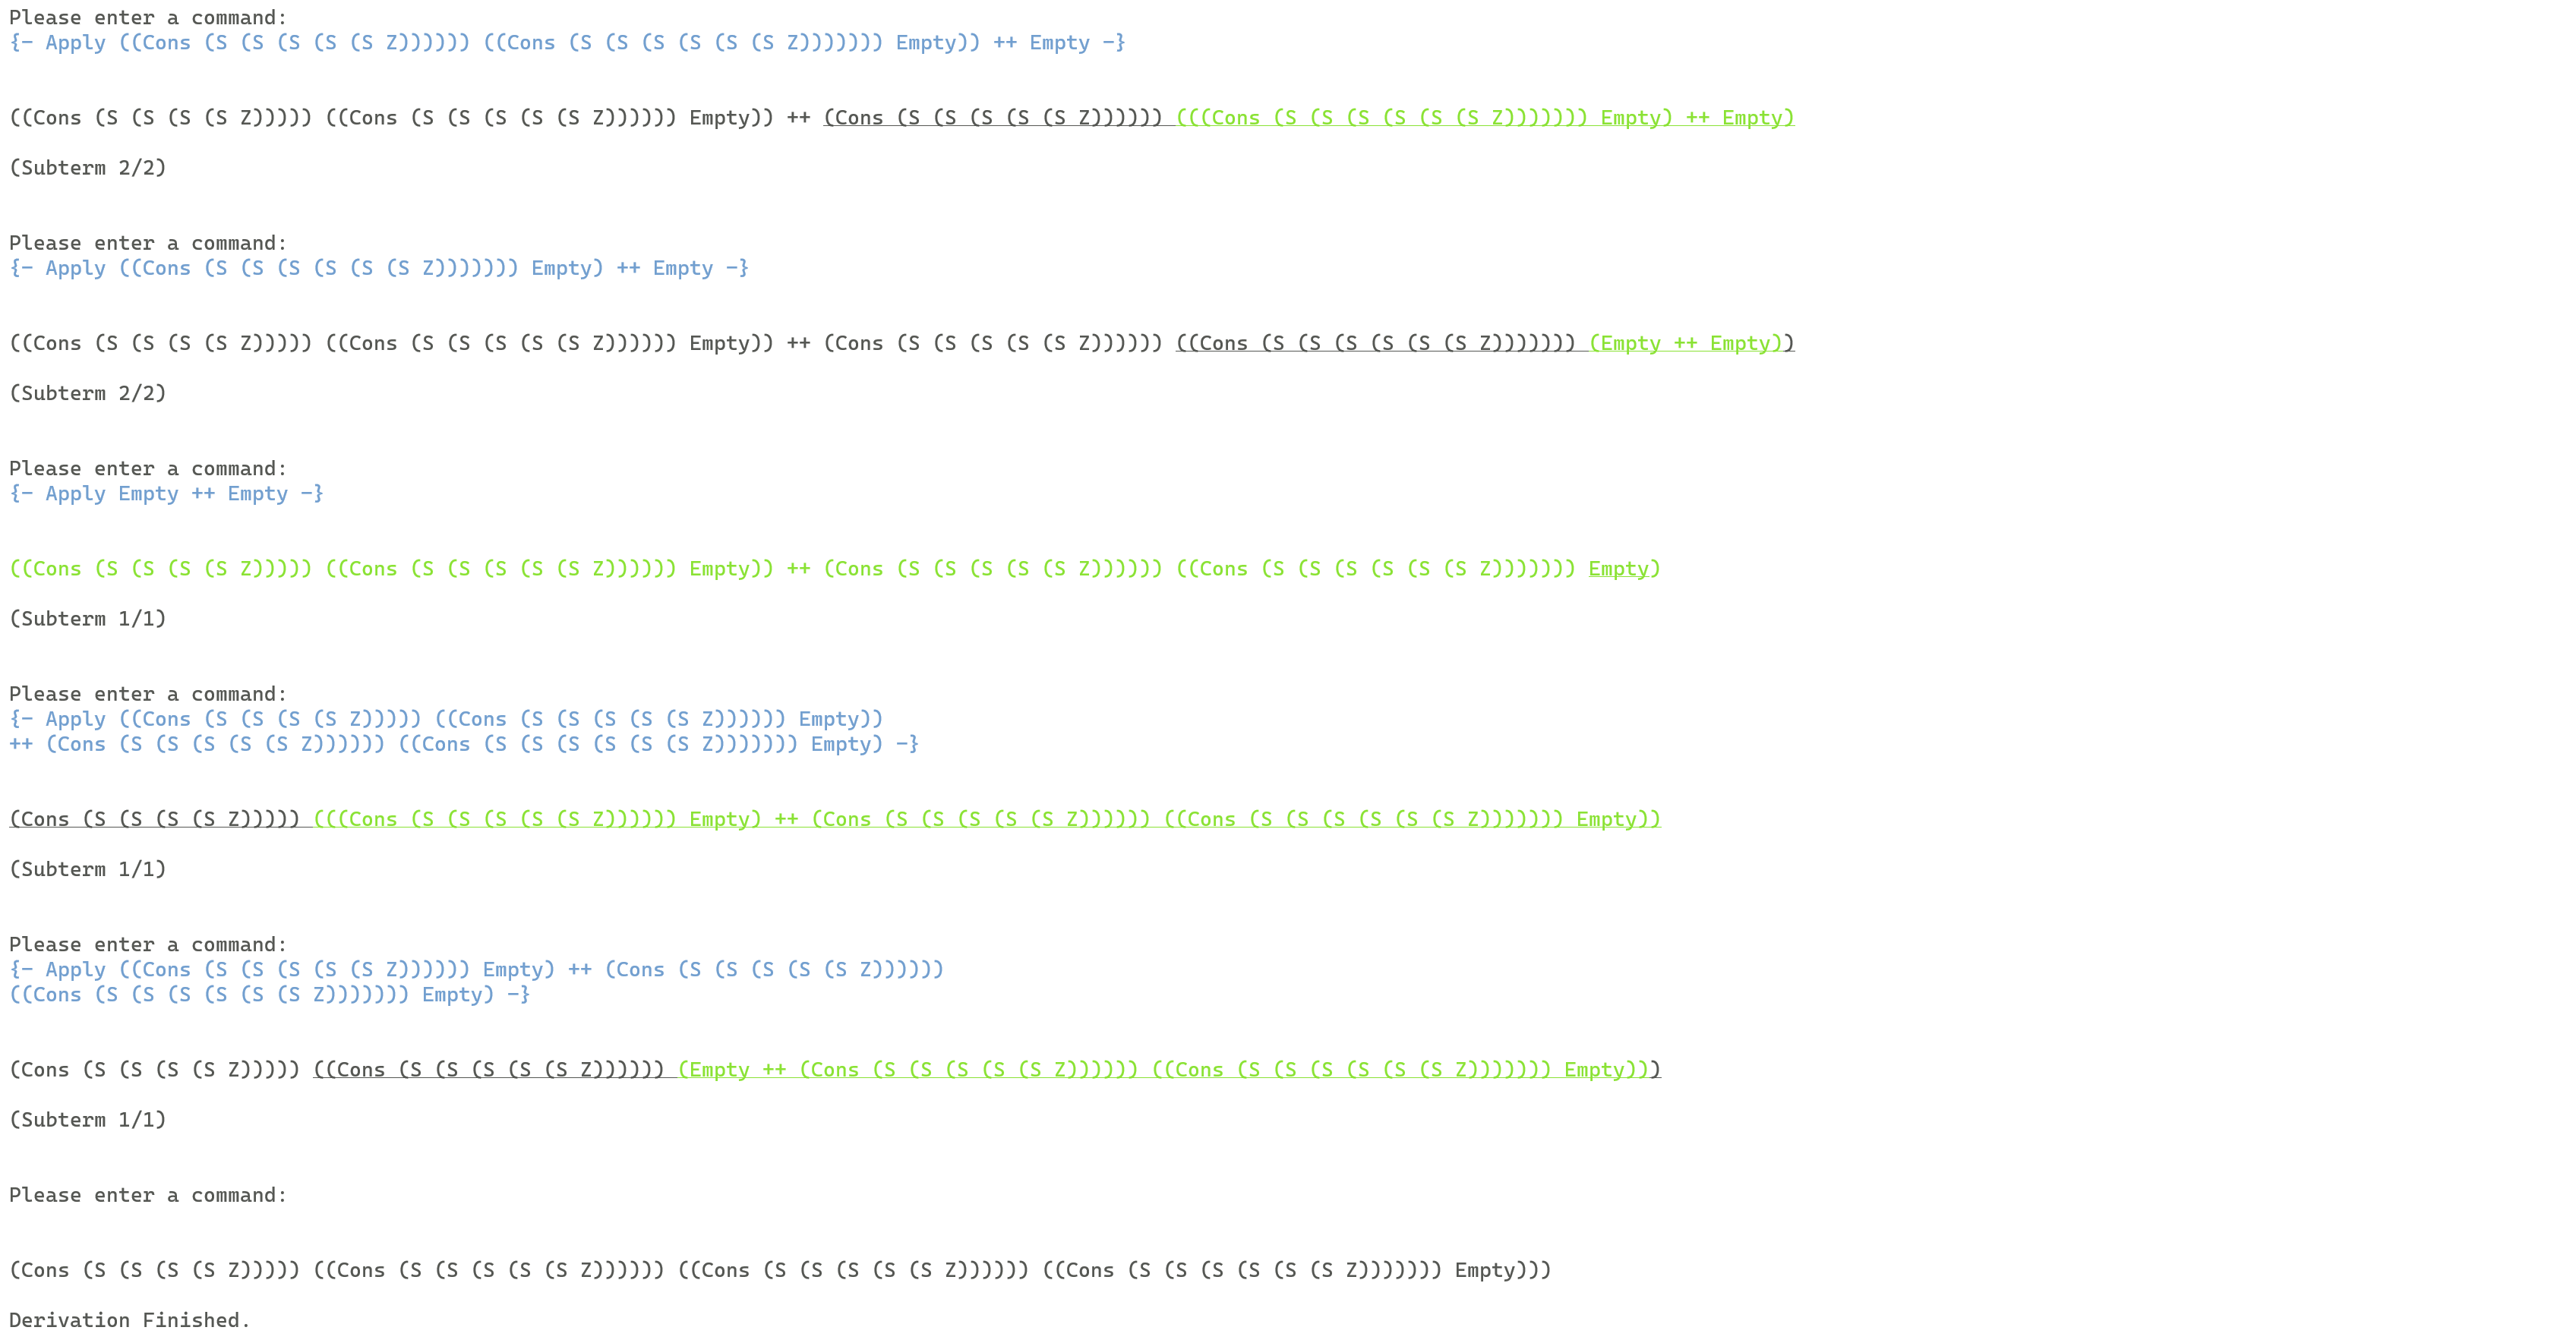
\includegraphics[width=1\textwidth]{resources/applicative_part_6.PNG}
    \caption{The third example, equivalent to \texttt{pure (+) <*> [1,2] <*> [3,4]}}
\end{figure}


\clearpage
\section{Example 4}
The fourth example needed to make a slightly bigger change again,
since it is using the Nat datatype as well.
Since division is harder to implement on the Nat datatype,
I have chosen to perform a subtraction instead.
Similar to the division for the Int datatype,
the subtraction for the Nat datatype can cause an error as well,
if a bigger number is subtracted from a smaller number (negative number error).

Because of this,
the fourth example here is pretty much equivalent to the example in the task description,
even though different operations and datatypes are used.

\begin{figure}
    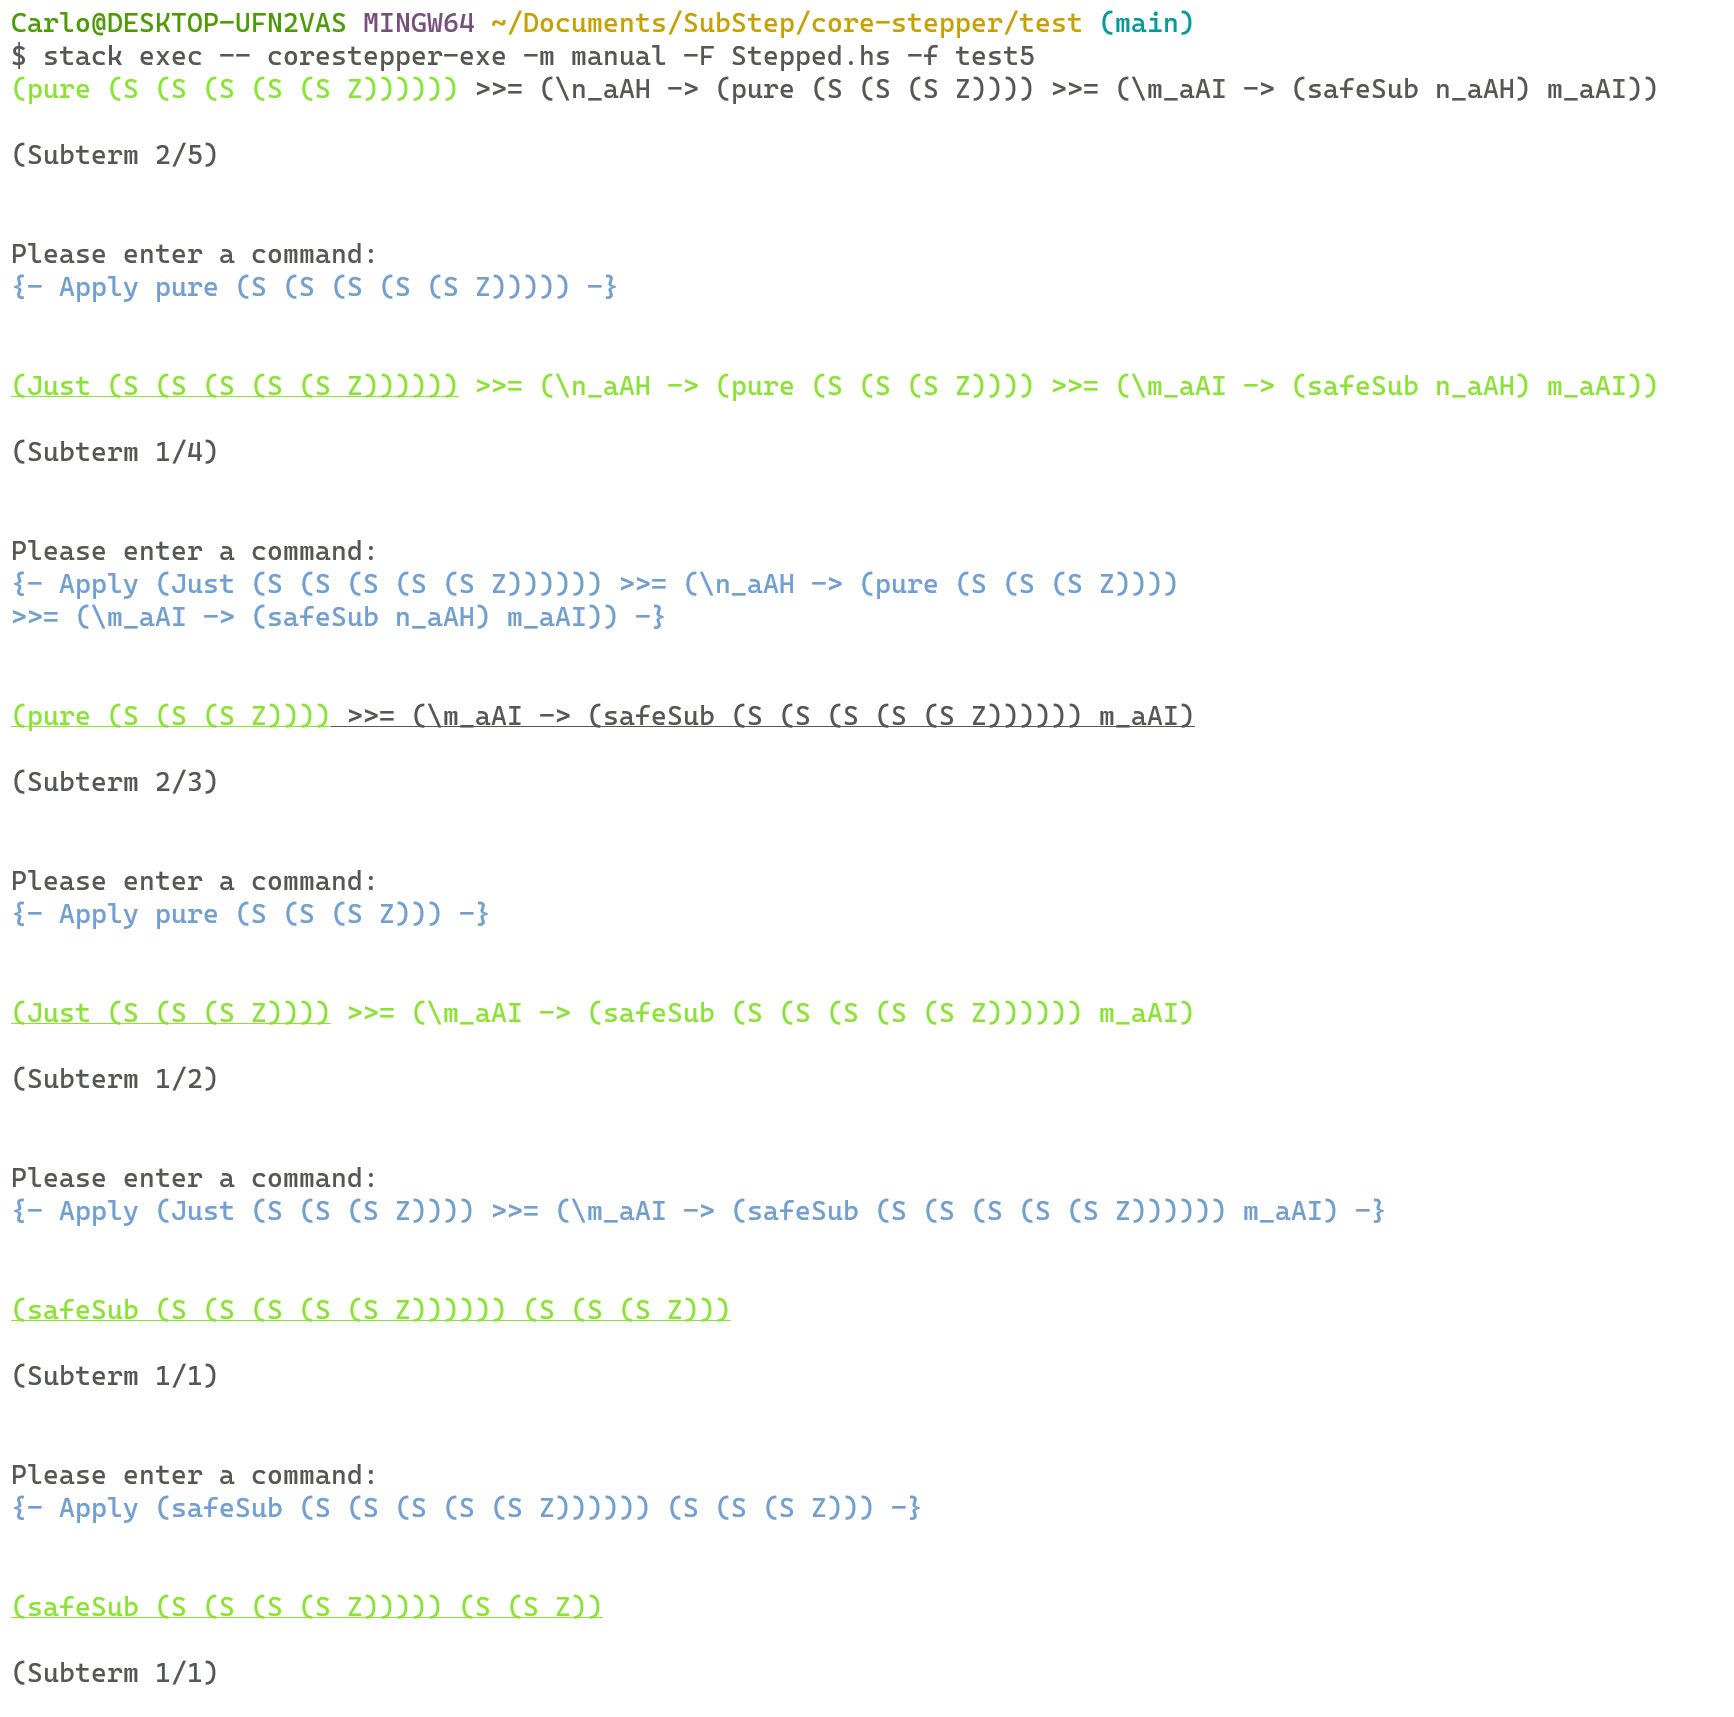
\includegraphics[width=1\textwidth]{resources/bind_part_1.PNG}
\end{figure}
\begin{figure}
    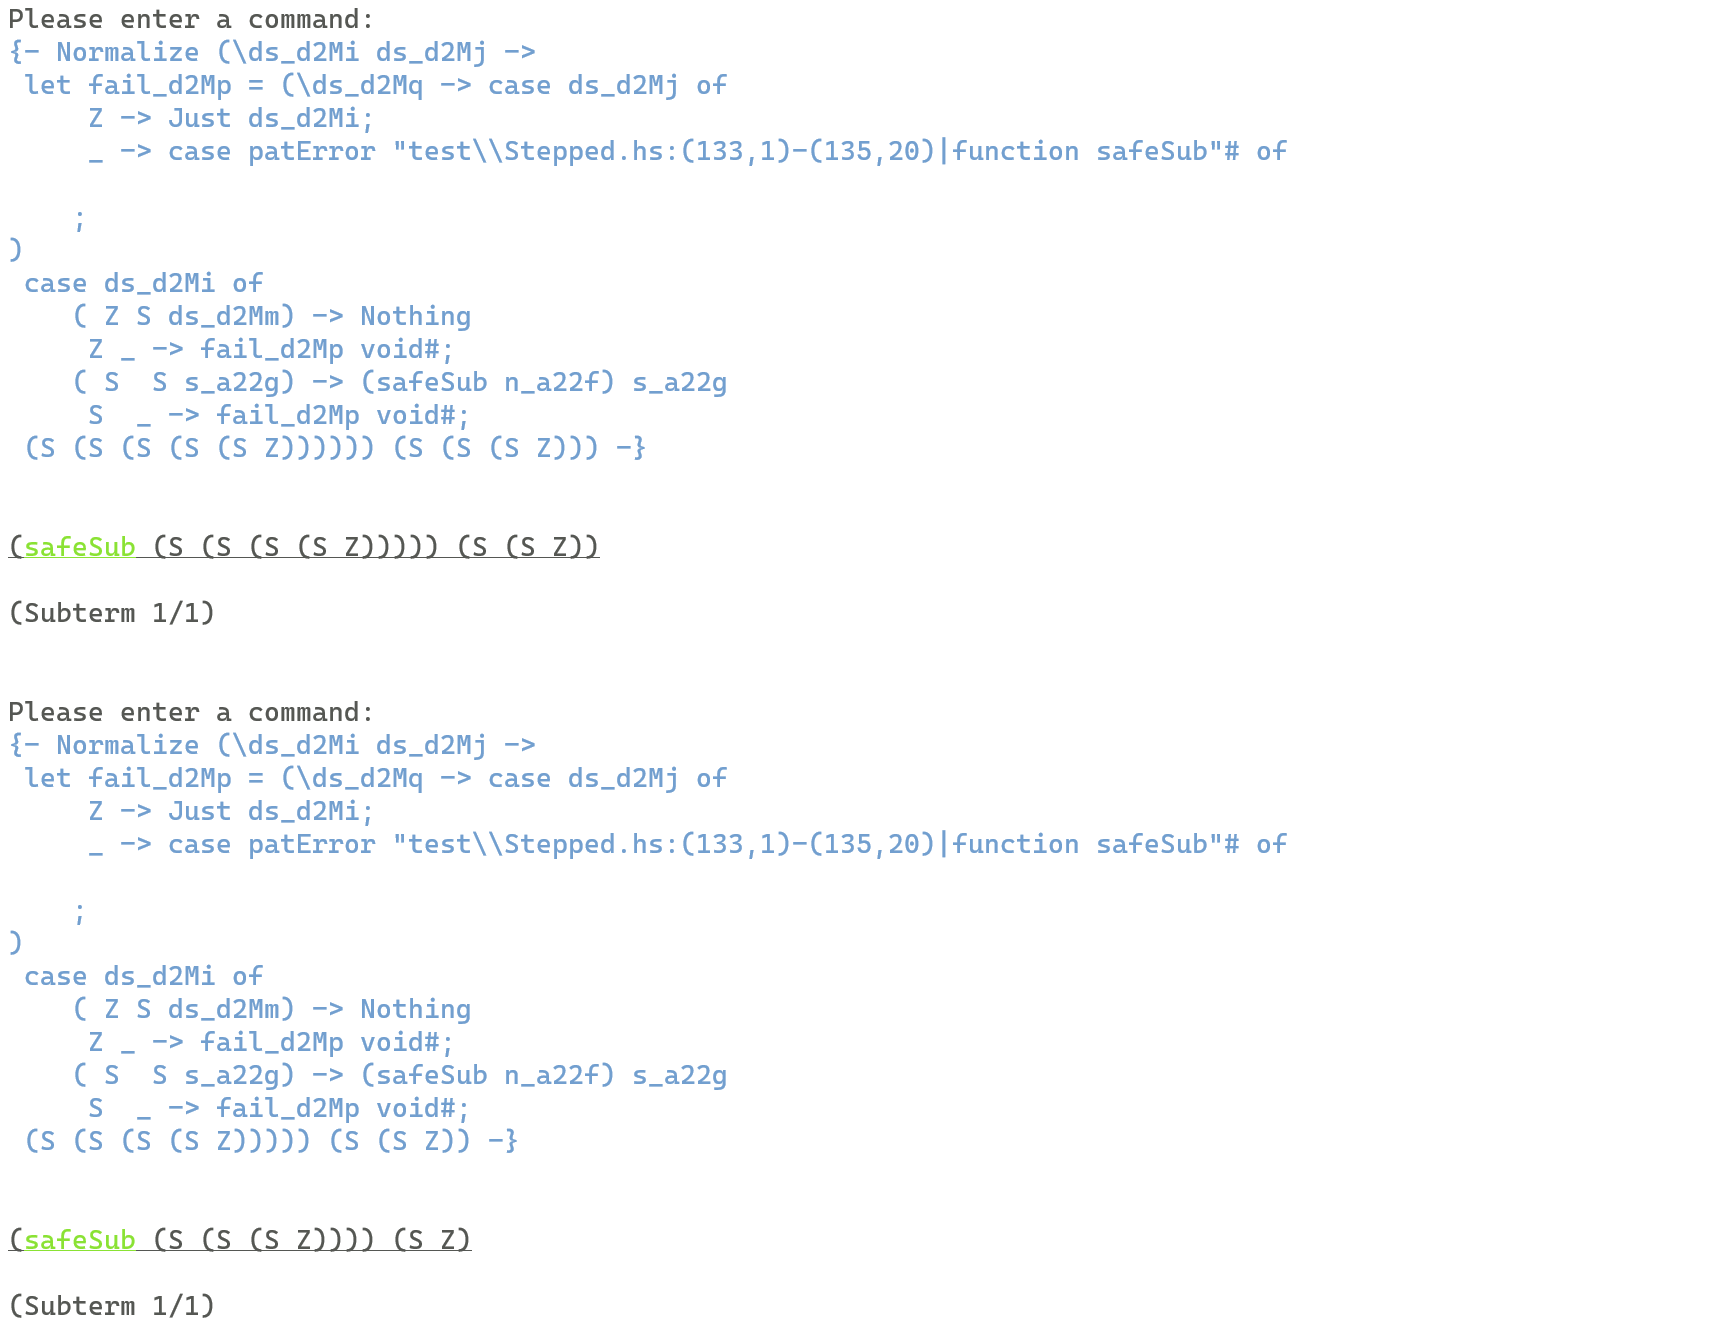
\includegraphics[width=1\textwidth]{resources/bind_part_2.PNG}
    \caption{The fourth example, equivalent to \texttt{\{do n <- 5; m <- 3; safeSub n m\}}}
\end{figure}

\chapter{Operational Notes}

\instructions{
    Vor allem bei Softwareprojekten: Gehen Sie auf folgende Punkte ein (bei grösserer Dokumentation
    verweisen Sie auf den Anhang).
    \begin{itemize}
        \item Verwendete SDK, IDE und Werkzeuge
        \item Hinweise zu CI/CD
        \item Installationsanleitung / Bedienungsanleitung
        \item Test-Logs
        \item Bei Systemen mit User Interfaces: Dokumentation der Usability Tests
    \end{itemize}
}


\section{CI/CD}

\subsection{Automated Documentation Building}

A GitHub Action that automatically builds a PDF from the \LaTeX-files has been created.
This ensures that the documentation can be easily accessed and viewed without requiring a \LaTeX-environment.
The first step (starting on line 11) compiles the document and creates a PDF.
The second step (starting on line 16) uploads the PDF so that it can be downloaded from the GitHub repository.

\begin{Verbatim}[samepage=true,numbers=left,xleftmargin=7.5mm]
name: Build LaTeX
on:
  push:
    branches: [ "main" ]
  workflow_dispatch:
jobs:
  build:
    runs-on: ubuntu-latest
    steps:
      - uses: actions/checkout@v3
      - name: Compile Document
        uses: xu-cheng/latex-action@v2
        with:
          working_directory: ./Documentation/src
          root_file: main.tex
      - name: Upload PDF
        uses: actions/upload-artifact@v3
        with:
          name: PDF
          path: ./Documentation/src/main.pdf
\end{Verbatim}


\section{Installation instructions}

\section{Test-logs}

            
\chapter{Personal Notes}
Working on this thesis was very enjoyable for me.
I appreciated the chance to work on a bigger project using Haskell.
It was extremely interesting to use such a different language for a change,
rather than building something using a language that I had used a lot in the past.

However,
it was also a bit of a challenge to work with somewhat unfamiliar technology.
While the functional programming class gave me an interesting overview of the basics and a bit more advanced topics like monads,
there was still much to learn.
I learned a lot about functional programming,
like how to use monad transformers and also other types of monads that were not covered in the lecture.
It was very cool that I got to put all these concepts, that were new to me, to use in this project.
I have gained a big appreciation for all the different monads,
that offer really helpful functionalities,
and especially the Maybe monad,
which makes the handling of failures beautifully elegant.

Of course,
it was not all sunshine and rainbows.
At the start of the project,
the hurdle of understanding Core and all the new concepts seemed hard to overcome.
There were times when I was a bit frustrated,
especially before I got to write some more lines of code and progress seemed slow.
However, once I started coding and things seemed to fall into place,
it was a lot of fun and it was really great to see how the project progressed steadily.

It was also a bit challenging to work on this thesis all by myself,
but I also enjoyed the ability to work at my own pace and not have to coordinate with a partner.
In addition, I also had the support of the previous developers of the Substitution Stepper,
which was very helpful at times and which I was really grateful for.
Of course, I also appreciated the valuable input that I have gotten from my advisor,
helping me to create a usable application.

Overall I am happy with the product that I created,
even though there are still some rough edges and things that could be improved.
I enjoyed being able to work on a project that I think could be really useful to my fellow students
and many other people trying to get into functional programming.


\end{document}
